\documentclass[11pt]{article}

% general text
\usepackage{color}


% about math
\usepackage{amsmath,amsthm}
\usepackage{amssymb,mathrsfs,amsfonts}
\usepackage{algorithm,algorithmicx,algpseudocode}
\usepackage{adjustbox}


% about graph & table
\usepackage{subfigure,tikz}
\usepackage{multirow,booktabs}
%\usepackage{array}
%\usepackage{rotating}


\usepackage[numbers]{natbib}
\usepackage{dcolumn}
\usepackage{arydshln}
\usepackage{enumitem}
\usepackage{rotating}

\usepackage{caption}
%\captionsetup[figure]{name=FIG.}
%\captionsetup[table]{name=TABLE}
\usepackage[labelsep=period]{caption}
%\usepackage{titlesec}
%\titlelabel{\thetitle.\quad}

\algdef{SE}[DOWHILE]{Do}{doWhile}{\algorithmicdo}[1]{\algorithmicwhile\ #1}%
%
\setlength{\textheight}{9.00in} \setlength{\textwidth}{6.50in}
\setlength{\oddsidemargin}{0.0in}
\setlength{\evensidemargin}{0.0in} \setlength{\topmargin}{0.0in}
\setlength{\headheight}{0in} \setlength{\headsep}{0in}
\setlength{\parindent}{0.25in} \setlength{\topskip}{0.0in}
\setlength{\marginparwidth}{.725in}


\newtheorem{theorem}{Theorem}
\newtheorem{definition}{Definition}
\newtheorem{lemma}{Lemma}
\newtheorem{corollary}{Corollary}
\newtheorem{conjecture}{Conjecture}
\newtheorem{remark}{Remark}
\newtheorem{proposition}{Proposition}
\newtheorem{assumption}{Assumption}
\newtheorem*{assumption*}{Assumption}
\newtheorem{example}{Example}


% These commands are new commands created by the author.
\renewcommand{\qedsymbol}{\rule{0.7em}{0.7em}}
\renewcommand{\baselinestretch}{1.0} % This sets the line spacing.  1.0 = single spaced, 2.0 = double spaced, etc.  Can use 1.25, etc.
%\DeclareMathSymbol{\mlq}{\mathord}{operators}{``}
%\DeclareMathSymbol{\mrq}{\mathord}{operators}{`'}


\newcommand{\tab}{\hspace{0.250in}}
\newcommand{\argmin}{\mathrm{argmin}}

\newcommand{\git}{\mathbin{
  \mathchoice{/\mkern-4mu/}% \displaystyle
    {/\mkern-4mu/}% \textstyle
    {/\mkern-4mu/}% \scriptstyle
    {/\mkern-4mu/}}}% \scriptscriptstyle

 \newcolumntype{d}[1]{D{.}{\cdot}{#1} }
 
 
 \newcommand{\RR}{\mathbb{R}}
 \newcommand{\ZZ}{\mathbb{Z}}
\newcommand{\EE}{\mathbb{E}} 
 \newcommand{\G}{\mathcal{G}}
 \newcommand{\N}{\mathcal{N}}
 \newcommand{\T}{\mathcal{T}}
 \newcommand{\X}{\mathcal{X}}
  \newcommand{\Pp}{\mathcal{P}}
  \newcommand{\Ss}{\mathcal{S}}
  \newcommand{\Aa}{\mathcal{A}}
  
 \newcommand{\conv}{\text{conv}}
\newcommand{\proj}{\text{proj}}






\title{A hierarchy bounds of bilevel mixed 0-1 programs}
%\author{Xueyu Shi$^1$, Bo Zeng$^1$, Oleg A. Prokopyev$^1$\footnote{Corresponding author. Email: droleg@pitt.edu; tel: +1-412-624-9833}}
%\institute{Industrial Engineering, University of Pittsburgh, 1048 Benedum Hall, Pittsburgh, Pennsylvania 15261}

%\date{November 2018}

\begin{document}

\maketitle

\begin{abstract}
	We consider general bilevel programs in which the decision variables of the lower-level problem are binary. A sequence of mixed-integer programming formulations are developed to obtain a hierarchy of bounds for the optimal objective function value of the bilevel programs. The proposed bounds are stronger to those provided by single-level relaxations. We then propose a family of valid inequalities based on mixing-set constraints to compute these bounds. Extended formulations are also explored to strengthen the formulations. Computational study indicates the efficiency of our bounds.
\end{abstract}

\section{Introduction}

The bilevel mixed-0,1 problem is given as follows:
\begin{align*}
[\text{BP}]~~	\eta^* = \max_{x\in \X}\; & \alpha_1^Tx + \alpha_2^Ty \\
	\text{s.t.~~} & y \in \underset{\hat{y}\in \{0,1\}^n}{\arg\max}\{\beta^T\hat{y}:\; Ax + B\hat{y} \leq d\} 
\end{align*}
where the feasible region of $x$ is a polyhedron $\X \subseteq \RR^{p_1} \times \ZZ^{p_2}$ and $A = (a_{i,j})_{m\times (p_1+p_2)}, B = (b_{i,j})_{m\times n}$. Let $\Pp = \{(x, y) \in \X \times \{0,1\}^n:\; Ax + By \leq d \}$, and denote $\Pp(x) = \{y \in \{0, 1\}^n:\; (x, y) \in \Pp \}$ as the feasible region of the follower with respect to the leader's decision $x$.  

However, in some situations, the follower might choose a local optimal solution and sacrifice his profit to benefit or damage the leader's objectives. In this note, we develop a hierarchy bounds for BP by considering the k-optimal solution of the lower-level problem. We say $y \in \Pp(x)$ is a k-optimal solution of the lower-level problem $LL(x)$, if $\beta^Ty$ is less than the objective of all neighborhood feasible solutions within $k$ distances, i.e., $\beta^Ty \geq \beta^T\hat{y}$ for all $\hat{y} \in \Pp(x)$ such that  $||y - \hat{y}||_1 \leq k$. Without loss of generality, we make the following assumptions throughout the paper.

\begin{assumption}
	The entries in $A, B, d$ are integers.
\end{assumption}
\begin{assumption}\label{assm:d_pos}
	The coefficients $\beta \geq 0$.
\end{assumption}
We note that the coefficients in $A, B, d$ can be transformed into integers as long as they are rational. As for Assumption \ref{assm:d_pos}, let $\hat{y}_j = 1-\hat{y}_j$ for any $\beta_j < 0$ and $j\in [n]:=\{1,2,\ldots, n\}$. The bilevel program with k-optimality for any positive integer $k$ is formalized as follows.
\begin{align*}
[\text{BP}_k]~~\eta_k^* = \max_{x, y}\; & \alpha_1^Tx + \alpha_2^Ty \\
\text{s.t.~~} &  (x, y)\in \Pp, \\
& d^T y \geq d^T \hat{y} \quad \forall\; \hat{y} \in \N^x_k(y),
\end{align*}
where $\N^x_k(y) = \{\hat{y} \in \Pp(x): ||\hat{y} - y||_1 \leq k \}$ denotes as the neighborhood of $y$ with distance $k$. Define the k-optimal reaction set of the follower with respect to the leader's decision $x$ as  
$$\Ss_k(x) = \{y\in \Pp(x): \beta^Ty \geq \beta^T\hat{y} \quad \forall\; \hat{y} \in \N^x_k(y)\}.$$ 
Note that $\Ss_0(x) = \Pp(x)$ for $k=0$, it follows that $\eta_0^*$ is the optimal objective function value of the single-level relaxation for the bilevel program.


Thus, we can establish progressively tighter upper bounds for the bilevel programs by increasing the neighborhood searching distance $k$.

\begin{proposition} \label{thm:hierachy_upper_bounds}
	$\eta_0^* \geq \eta_1^* \geq \eta_2^* \geq \cdots \geq \eta_n^* = \eta^*$.  
\end{proposition}
\begin{proof}
	Note that $\eta_k^* = \max_{x, y}\; \{\alpha_1^Tx + \alpha_2^Ty:  (x, y) \in \Pp, y\in \Ss_k(x)\}$. To prove $\eta_k^* \geq \eta_{k+1}^*$ for $k=0, 1, \ldots, n-1$, it suffices to show that $\Ss_{k}(x) \supseteq \Ss_{k+1}(x)$. For any solution $y \in \Ss_{k+1}(x)$, then $\beta^T y \geq \beta^T \hat{y}$ for all $\hat{y} \in \N^x_{k+1}(y)$. Observe that $\N^x_{k+1}(y) \supseteq \N^x_{k}(y)$, thus $\beta^T y \geq \beta^T \hat{y}$ for all $\hat{y} \in \N^x_{k}(y)$, which implies that $y\in \Ss_k(x)$.
	
	If $k = n$, then $\N^x_n(y) = \Pp(x)$. For any solution $y\in \Ss_n(x)$, then $\beta^T y \geq \beta^T \hat{y}$ for all $\hat{y} \in \Pp(x)$. It follows that $\Ss_n(x) = \underset{\hat{y}}{\arg\max}\{\beta^T\hat{y}:\; \hat{y} \in \Pp(x)\}$ and $\eta_n^* = \eta^*$.
\end{proof}

\begin{theorem}
	BP$_k$ is NP-hard for $k\geq2$.
\end{theorem}
\begin{proof}
	Consider the minimum spanning tree interdiction problem \cite{frederickson1999increasing} to find the most vital arcs whose removal increase the weight of minimum spanning tree as large as possible. Formally, given a graph $G = (V, E)$ with edge weight vector $w\in \RR_+^{|E|}$. Then the minimum spanning tree interdiction problem is given as
	\begin{align*}
		\max_{x\in \{0,1\}^E}&  \min_{y\in \{0,1\}^E} w^Ty \\
		&  \sum_{i} x_i \leq k, \\
		&  y \in \mathcal{T}(G), \\
		&  y \leq 1 - x,
	\end{align*} 
	where $\mathcal{T}(G)$ is the set of incidence vectors for the spanning trees in $G$. \citet{frederickson1999increasing} show the NP-hardness of the above problem. Note that for the minimum spanning tree problem, any 2-optimal solution is a global minimum due to the matroid property. Therefore, the minimum spanning tree interdiction problem when the follower takes k-optimal solutions for $k\geq 2$ is equivalent to the minimum spanning tree interdiction problem. It follows that BLKOP is NP-hard in general. 
\end{proof}


The bilevel programming is known as the NP-hard problem. The common method for the bilevel linear programming is to reformulate into a single-level mixed-integer problem by using KKT conditions. However, there do not have efficient solvers for the bilevel mixed-integer problem. The branch-and-cut approach has been investigated broadly to solve the bilevel mixed-integer problem. In this paper, we  formulate the bilevel problem with k-optimality as a single-level problem, and investigate the general framework to obtain tighter upper bounds for the bilevel mixed 0-1 problems. Furthermore, the proposed framework can be used in the following manners:
\begin{itemize}
	\item By solving bilevel problem with k-optimality, we can obtain a near-optimal leader's decisions. By increasing the number of $k$, the tighter upper and lower bounds can be obtained but generally more difficult to compute.
	\item The single-level relaxation is mostly used formulation in the branch-and-cut approach. The bilevel problem with k-optimality provides tighter relaxation methods that can be embedded into the general branch-and-cut framework.
	\item For the bilevel problem in which any k-optimal solution is a global optima for the lower-level problem, then the proposed framework provides a single-level reformulation for these bilevel problems. We would show that the minimum spanning tree interdiction problem can be reformulated into a single-level mixed-integer problem.
	\item Practically, it is difficult for the followers to choose their global optimal solution due to the computational complexity. The reaction solution set of the follower might be the local optima of the lower-level problem. The bilevel problem with k-optimality actually considers that the k-optimal solution is selected for the follower. 
\end{itemize} 


\noindent\textbf{Notation.} Denote set $[n] = \{1, 2, \ldots, n\}$ for any positive integer $n$. 


\section{The bilevel problem with $k$-optimality}
In this section, we propose to formulate $BP_k$ into a single-level mixed-integer problem. A general branch-and-cut approach is then developed to solve the problem.

\subsection{$k = 1$ case}

When $k=1$, then recall the 1-optimal reaction set of the follower is:
\[\Ss_1(x) = \{y \in \Pp(x): \beta^T y \geq \beta^T \hat{y} \quad \forall\; \hat{y} \in \N^x_1(y)\},\]
where $\N^x_1(y) = \{\hat{y} \in \Pp(x): ||\hat{y} - y||_1 \leq 1 \}$. An equivalent condition of $y\in \Ss_1(x)$ is given:
\begin{lemma}\label{thm:opt_condition_k1}
	Given a solution $(x, y) \in \Pp$, then $y\in \Ss_1(x)$ if and only if either $y_j = 1$, or $y_j = 0$ and $y + e_j \notin \Pp(x)$ for $j\in I_\beta^+$,  where $e_j$ is the $j$th unit vector, and $I_\beta^+ = \{j \in [n]: \beta_j >0\}$.
\end{lemma}

Follows from Lemma \ref{thm:opt_condition_k1}, a sufficient condition is given that the bilevel problem with 1-optimality is equivalent to the single-level relaxation.

\begin{proposition} \label{thm:hpp=1optimal}
	If $\alpha_{2j} > 0$ for all $j\in I_\beta^+$, then $\eta_0^* = \eta_1^*$.
\end{proposition}
\begin{proof}
	Based on Proposition \ref{thm:hierachy_upper_bounds}, we have $\eta^*_0 \geq \eta^*_1$. Thus, we only need to prove that $\eta^*_0 \leq \eta^*_1$. Suppose $(x^*, y^*)$ is an optimal solution of single-level relaxation problem, it suffices to show that $(x^*, y^*)$ is also a feasible solution for BP$_1$, that is $y^* \in \Ss_1(x^*)$. We first note that $y^* \in \Pp(x^*)$.
	
	Suppose $y^* \notin \Ss_1(x^*)$, then based on Lemma \ref{thm:opt_condition_k1}, there exists some $j \in I^+_\beta$ such that $y^*_j = 0$ and $y^*+e_j \in \Pp(x)$. Let $y' = y^* + e_j$, then $(x^*, y')$ is a feasible solution of the single-level relaxation problem. Since $\alpha_{2j} > 0$ for $j \in I_\beta^+$, then $\alpha_1x^* + \alpha_2y' = \alpha_1x^* + \alpha_2y^* + \alpha_{2j} > \alpha_1x^* + \alpha_2y^*$, which contradicts with the fact that $(x^*, y^*)$ is an optima. Therefore, $y_1^* \in \Ss_1(x^*)$, and the result follows.
	
	
\end{proof}


Through Proposition \ref{thm:hpp=1optimal}, we can establish the NP-hardness of BP$_k$ for $k=1$.
\begin{theorem}
	BP$_k$ is NP-hard for $k=1$.
\end{theorem}
\begin{proof}
	Consider the bilevel knapsack problem proposed in \cite{mansi2012exact}, 
	\[ \max_{x\in \{0,1\}^m}\Big\{c^1x + c^2y: y \in \arg\max_{y\in \{0,1\}^n}\{ dy: a^1x + a^2 y \leq b \} \Big\}, \]
	where $c^i, d, a^i$ are nonnegative integral vectors, and $b\in \ZZ_+$. From Proposition \ref{thm:hpp=1optimal}, we have that $BP_k$ with $k=1$ is equivalent to the single-level relaxation problem, which is a knapsack problem given by
	\[\max_{x, y}\Big\{c^1x + c^2y: a^1x + a^2 y \leq b, x\in \{0,1\}^m, y\in \{0,1\}^n \Big\}. \]
	It is known the fact that the knapsack is NP-hard in general, then the result follows.
\end{proof}


We next focus on the single-level formulation for the bilevel problem with 1-optimality. Observe that for any solution $y \in \{0,1\}^n$, if $y \notin \Pp(x)$, then there must exist some row $i\in [m]$ such that 
\[\sum_{j} a_{i,j} x_j + \sum_{j} b_{i,j} y_j \geq d_i + 1,  \]
which yields that
\[\Big\{y\in \{0,1\}^n: y\notin \Pp(x) \Big\} = \bigcup_{i=1}^m \Big\{y\in \{0,1\}^n: \sum_{j} b_{i,j} y_j \geq b_i + 1 -  \sum_{j} a_{i,j} x_j  \Big\}.\]

To formulate the constraints that $y+e_j \notin \Pp(x)$ for $j\in I_\beta^+$ and $y_j = 0$, we introduce binary variables that $z_{i,j} = 0, j \in I_\beta^+$ indicates the $i$th row is violated by $y+e_j$ for $j\in I_\beta^+$.  Then we reformulate BP$_1$ as a mixed-integer linear problem:

\begin{align}
[\text{BP}_1]~~\eta_1^* = \max_{x, y, z}\; & \alpha_1^Tx + \alpha_2^Ty \nonumber \\
\text{s.t.~~} &  (x, y)\in \Pp, \nonumber \\
& \sum_{j=1}^n a_{i,j} x_j + \sum_{j=1}^n b_{i,j} y_j + (h_{i,j} - \mu_i)z_{i,j} \geq h_{i,j} \quad i \in [m], j\in I_\beta^+, \label{eq:K1_1} \\
& \sum_{i=1}^m z_{i,j} - y_j = m - 1  \quad j\in I_\beta^+, \label{eq:K1_2} \\
& z_{i,j} \in \{0,1\} \quad i \in [m], j\in I_\beta^+, \nonumber
\end{align}
where $h_{i,j} = d_i + 1 - b_{i, j}$, and $\mu_i$ is a sufficiently small constant. Given the bound of $x$ that $\ell_j \leq x_j \leq u_j$ for any $j$, then we have for $i$th constraint:
\[\sum_{j=1}^n a_{i,j} x_j + \sum_{j=1}^n b_{i,j} y_j \geq \sum_{j: a_{i,j} > 0} \ell_j + \sum_{j:a_{i,j}<0}u_j + \sum_{j:b_{i,j}<0} 1. \]
Then we can set $\mu_i = \sum_{j: a_{i,j} > 0} \ell_j + \sum_{j:a_{i,j}<0}u_j + \sum_{j:b_{i,j}<0} 1$. Constraints \eqref{eq:K1_1} ensure that if $z_{i,j} = 0$, then $y + e_j$ violates $i$th constraint, otherwise if $z_{i,j} = 1$, then the $i$th constraint for $y + e_j$ is not considered. Constraints \eqref{eq:K1_2} guarantee that if $y_j = 0$, then there exits some $i$ such that $z_{i,j} = 0$ which implies that the $i$th constraint is violated by $y+e_j$ and $y+e_j \notin \Pp(x)$. Otherwise if $y_j = 1$, then $z_{i,j} = 1$ for all $i \in [m]$ and constraints \eqref{eq:K1_1} are always satisfied.  Next, we discuss how to reduce the number of variables by preprocessing.
\begin{proposition}
	If $\alpha_{2,j_0} > 0$ and $b_{i, j_0} \geq 0$ for some $j_0\in I_\beta^+$ and all $i\in [m]$, then it is equivalent to compute $\eta_1^*$ by removing variables $z_{i, j_0}$ and the corresponding constraints.
\end{proposition}
\begin{proof}
	Denote BP$_1'$ and $\eta_1'$ as the problem by setting $z_{i_0, j_0}=1$ and its optimal objective function value, respectively. It is clear that $\eta_1' \geq \eta_1^*$. Assume $(x', y', z')$ is the optimal solution of BP$_1'$, then we show that $y' \in \Ss_1(x')$, which implies that $(x', y')$ is feasible for BP$_1$. It immediately results in $\eta_1' \leq \eta_1^*$. Note that to check $y' \in \Ss_1(x')$, it suffices to show that $y'+e_{j_0} \notin \Pp(x)$.
	
	If $y_{j_0}' = 1$, then the statement holds trivially. If $y_{j_0}' = 0$, then suppose $y' + e_{j_0} \in \Pp(x)$.  For those $j\in [n]$ and $y'_j=0$, then we have $y' + e_{j_0} + e_j \notin \Pp(x)$ due to $b_{i, j_0} \geq 0$ for all $i$. Therefore, $y'+e_{j_0}$ is a feasible solution in BP$'_k$. Also, $\alpha_1^Tx' + \alpha_2^T(y'+e_j) = \alpha_1^Tx' + \alpha_2^Ty' + \alpha_{2j} > \alpha_1^Tx' + \alpha_2^Ty'$, which contradicts with the assumption that $(x', y', z')$ is an optima of BP$_1'$. Thus, $y' + e_j \notin \Pp(x)$ and the result follows.
\end{proof}

\noindent\textbf{Preprocessing:} \begin{itemize}
	\item If $b_{i,j} \leq 0$ for some $i\in [m]$ and $j\in I_\beta^+$, then we can set $z_{i, j} = 1$. 
	\item If $b_{\cdot, j_1} \leq b_{\cdot, j_2}$ for some $j_1, j_2\in [n]$, then we can strengthen constraints \eqref{eq:K1_2} for $j_2$ as 
	\[  \sum_i z_{i,j_2} - y_{j_1}y_{j_2} + y_{j_1}  = m. \]
\end{itemize}


We next focus on the valid inequalities of BP$_1$. Let $\pi_i =  \sum_{j=1}^n a_{i,j} x_j + \sum_{j=1}^n b_{i,j} y_j$ for $i\in [m]$, then constraints \eqref{eq:K1_1} become
\[ \pi_i + (h_{i, j} - \mu_i) z_{i,j} \geq h_{i, j} \quad \forall i\in [m], j\in I_\beta^+. \]

Note that the above inequalities are called mixing set constraints, which have been extensively studied by \cite{gunluk2001mixing,atamturk2000mixed,luedtke2010integer,kuccukyavuz2012mixing,abdi2016mixing,zhao2017polyhedral}. Furthermore, the convex hull of $\{(\pi, z)\in \RR\times \{0,1\}^n: \pi + h_jz_j \geq h_j\}$ is sufficiently described by the star inequalities
\[ \pi + \sum_{j=1}^l (h_{t_j} - h_{t_{j+1}}) z_{t_j} \geq h_{t_1} \]
where $h_{1} \geq \cdots \geq h_n$ and $t_1 < \cdots < t_l, h_{t_{l+1}} = 0$. Similarly, we can propose a family of valid inequalities for BP$_1$. 
\begin{proposition}\label{thm:k_1_valid}
	Given some $i\in [m]$, we assume $I_\beta^+ = \{1, \ldots, |I_\beta^+|\}$ and $b_{i,1} \leq \cdots \leq b_{i,|I_\beta^+|}$, then the following inequalities
	\begin{equation}\label{eq:k_1_star}
		\sum_{j=1}^n a_{i,j} x_j + \sum_{j=1}^n b_{i,j} y_j  + \sum_{j=1}^{l} (h_{i,t_j} - h_{i,t_{j+1}}) z_{i,t_j} \geq h_{i, t_1} \quad \forall \{t_1, \ldots, t_l\} \subseteq I_\beta^+
	\end{equation}
	are valid for the feasible region of BP$_1$, where $h_{i,t_{l+1}} = \mu_i.$ Furthermore, if $h_{i, t_1} < h_{i, 1}$, we can strengthen the above inequality by containing $1$ in the set.
\end{proposition}
\begin{proof}
	The result follows directly from \cite{gunluk2001mixing,luedtke2010integer}. However, since our formulations are somewhat different, we provide a self-contained proof. Let $(x, y, z)$ be a feasible solution of BP$_1$. Remind that in constraint \eqref{eq:K1_1}, if $z_{ij}=0$ for some $j\in [n]$, then $\sum_{j=1}^n a_{i,j} x_j + \sum_{j=1}^n b_{i,j} y_j \geq h_{i,j}$.  
	
	For any $\{t_1, \ldots, t_l\} \subseteq I_\beta^+$ and $i\in [m]$, if $z_{i, t_j} = 1$ for all $j \in \{1, \ldots, l\}$, then the inequality \eqref{eq:k_1_star} always holds as $\sum_{j=1}^n a_{i,j} x_j + \sum_{j=1}^n b_{i,j} y_j \geq \mu_i$. If there exists $z_{i,t_j}=0$ for some $j\in \{1, \ldots, l\}$, let $j^*=\min\{j\in \{1, \ldots, l\}:\; z_{i,t_j}=0\}$. Thus, $\sum_{j=1}^n a_{i,j} x_j + \sum_{j=1}^n b_{i,j} y_j \geq h_{i,t_{j^*}}$ and 
	\begin{align*}
		\sum_{j=1}^n a_{i,j} x_j + \sum_{j=1}^n b_{i,j} y_j  + \sum_{j=1}^{l} (h_{i,t_j} - h_{i,t_{j+1}}) z_{i,t_j} & \geq \sum_{j=1}^n a_{i,j} x_j + \sum_{j=1}^n b_{i,j} y_j + \sum_{j=1}^{j^*} (h_{i,t_j} - h_{i,t_{j+1}}) z_{i,t_j} \\
		& = \sum_{j=1}^n a_{i,j} x_j + \sum_{j=1}^n b_{i,j} y_j + \sum_{j=1}^{{j^*-1}} (h_{i,t_j} - h_{i,t_{j+1}}) \\
		& = \sum_{j=1}^n a_{i,j} x_j + \sum_{j=1}^n b_{i,j} y_j + h_{i, t_1} - h_{i,t_{j^*}}\\
		& \geq h_{i, t_1}.
	\end{align*}
	If $h_{i, t_1} < h_{i, 1}$, and we add $1$ to the set, then firstly based on the above discussion, we have that the inequality 
	\begin{equation} \label{eq:K_1_star2}
		\sum_{j=1}^n a_{i,j} x_j + \sum_{j=1}^n b_{i,j} y_j  + (h_{i, 1}-h_{i, t_1}) z_{i, 1} +   \sum_{j=1}^{l} (h_{i,t_j} - h_{i,t_{j+1}}) z_{i,t_j} \geq h_{i, 1}
	\end{equation} 
	is valid for BP$_1$. Since $h_{i, 1} - (h_{i, 1}-h_{i, t_1}) z_{i, 1} = h_{i, 1} (1-z_{i, 1}) + h_{i, t_1} z_{i, 1} >  h_{i, t_1}$, the inequality \eqref{eq:K_1_star2} is stronger than \eqref{eq:k_1_star}.
	
\end{proof}


\subsection{General k}
Let $\T_k = \{ (T_1, T_2)\subseteq [n]\times [n]: T_1\cap T_2 = \emptyset, \beta(T_1) > \beta(T_2), |T_1\cup T_2|=k\}$. We first provide an equivalent condition for $\Ss_k(x)$. 
\begin{lemma}\label{thm:opt_condition_k}
	For any $x\in X$, then $y\in \Ss_k(x)$ if and only if the following conditions are satisfied:
	\begin{itemize}
		\item[\emph{(i)}] $y\in \Ss_{k-1}(x)$; 
		\item[\emph{(ii)}] For any $(T_1, T_2) \in \T_k$, if $y_j = 0$ for $j\in T_1$ and $y_j = 1$ for $j\in T_2$, then $y + \sum_{j\in T_1} e_j - \sum_{j\in T_2} e_j \notin \Pp(x)$.
	\end{itemize}
\end{lemma}

\begin{proposition}
	If $\alpha_2(T_1) > \alpha_2(T_2)$ for any $(T_1, T_2) \in \cup_{j=1}^k \T_j$, then $\eta^*_k = \eta^*_{k-1} = \cdots = \eta^*_0$.
\end{proposition}
\begin{proof}
	Based on Proposition \ref{thm:hierachy_upper_bounds}, we have $\eta^*_0 \geq \cdots \geq \eta^*_{k-1} \geq \eta^*_k$. Thus, we only need to prove that $\eta^*_0 \leq \eta^*_k$. Suppose $(x^*, y^*)$ is an optimal solution of $BP_{0}$, it suffices to show that $(x^*, y^*)$ is also a feasible solution for $BP_k$, that is $y^* \in \Ss_k(x^*)$. We first note that $y^* \in \Pp(x^*)$ and $\alpha_2 y^* \geq \alpha_2 y$ for any $y \in \Pp(x^*)$.
	
	Suppose $y^* \notin \Ss_k(x^*)$, then based on Lemma \ref{thm:opt_condition_k}, there exists $(T_1, T_2) \in \cup_{j=1}^k \T_j$ such that $y^*_j = 0$ for $j\in T_1$, $y^*_j = 1$ for $j\in T_2$ and $y + \sum_{j\in T_1} e_j - \sum_{j\in T_2} e_j \in \Pp(x)$.  Since $\alpha_2(T_1) > \alpha_2(T_2)$, then $\alpha_2 y + \alpha_2(T_1) - \alpha_2(T_2) > \alpha_2y$, which contradicts with the assumption that $(x^*, y^*)$ is optima for $BP_0$. Therefore, $y\in \Ss_k(x^*)$ and the result follows.
\end{proof}


To interpret the conditions in Lemma \ref{thm:opt_condition_k} into the constraints, we introduce binary variables $z_{i,t}$ for $i\in [m]$ and $t=(T_1, T_2) \in \T^k=\cup_{j=1}^k \T_k$. Then the $BP_k$ is reformulated as 
\begin{align}
[BP_k]~~\eta_k^* = \max_{x, y, \pi, z}\; & \alpha_1^Tx + \alpha_2^Ty \nonumber \\
\text{s.t.~~} &  (x, y)\in \Pp, \nonumber \\
& \pi = Ax + By,  \label{eq:BP_k_1}\\
& \pi_i + (h_{i,t} - \mu_i) z_{i,t} \geq h_{i,t} ~\forall i \in [m], t\in \T^k, \label{eq:BP_k_mixing} \\
& \sum_{i=1}^m z_{i,t} + \sum_{j\in T_2} (y_j-1) - \sum_{j\in T_1}y_j \leq m-1  \; \forall t = (T_1, T_2)\in \T^k, \label{eq:BP_k_2}\\
& \sum_{i=1}^m z_{i,t} \geq m -1 \quad \forall t\in \T^k, \label{eq:BP_k_3}\\
& z_{i,t} \in \{0, 1\}\quad \forall i\in [m], t\in \T^k,
\end{align}
where $h_{i,t} = b_i + 1 - (\sum_{j\in T_1} b_{i,j}  - \sum_{j\in T_2} b_{i,j})$ for any $t = (T_1, T_2)\in \T^k.$ Note that for the fixed $k$, the cardinality of $\T^k$ is $O(n^k)$, which implies that the reformulation is polynomial-time reducible from BP$_k$. Furthermore, we can decrease the included variables and constraints through preprocessing process.\\


\begin{proposition}
	\begin{itemize}
		\item[\emph{(i)}] If $\sum_{j\in T_1} b_{i,j}  - \sum_{j\in T_2} b_{i,j} \leq 0$ for some $t = (T_1, T_2)\in \T^k$ and $i\in [m]$, then we can set $z_{i, t} = 1$.
		\item[\emph{(ii)}] Given some $t_1=(T_1, T_2) \in \T^{k-1}$ and $j \in [n]\setminus (T_1\cup T_2)$. Let $t_2 = (T_1\cup \{\ell\}, T_2) \in \T^k$, if $b_{i,\ell} \geq 0$ for all $ i\in [m]$, then we can remove variable $z_{i, {t_2}}$ and its corresponding constraints.
		\item[\emph{(iii)}]  Given some $t_1=(T_1, T_2) \in \T^{k-1}$ and $j \in [n]\setminus (T_1\cup T_2)$. Let $t_2 = (T_1, T_2\cup \{\ell\}) \in \T^k$, if $b_{i,\ell} \leq 0$ for all $ i\in [m]$, then we can remove variable $z_{i, {t_2}}$ and its corresponding constraints. 
		\item[\emph{(iv)}] If $h_{i,t_1} = h_{i, t_2}$ for some $i\in [m]$ and $t_1, t_2\in \T^k$, then replace $z_{i, t_2}$ as $z_{i, t_1}$ in the model.
		\item[\emph{(v)}] If $\alpha_2(T_1) > \alpha_2(T_2)$ for some $t = (T_1, T_2) \in \T^k$, and $\sum_{j\in T_1} a_{i,j} \geq \sum_{j\in T_2} a_{i,j}$ for all $i\in [m]$, then we can remove $z_{i,t}$ for all $i$ and its corresponding constraints.
	\end{itemize}
\end{proposition}
\begin{proof}
	\begin{itemize}
		\item[(i)] It is sufficient to show that $z_{i,t} = 1$ for any feasible solution $(x, y, z)$ for BP$_k$.  Since $(x, y) \in \Pp$, then $\pi_i \leq b_i$. If $z_{i,t} = 0$, then according to constraint \eqref{eq:BP_k_mixing}, we have 
		\[\pi_i \geq b_i + 1 - (\sum_{j\in T_1}b_{i,j} - \sum_{j\in T_2} b_{i, j}) \geq b_i + 1, \]
		where the second inequality follows from the assumption that $\sum_{j\in T_1} b_{i,j}  - \sum_{j\in T_2} b_{i,j} \leq 0$. Thus, we obtain a contradiction. It is immediate that $z_{i,t}$ should equal to $1$.
		
		\item[(ii)] Denote $BP_k'$ and $\eta_k'$ as the problem by removing variables $z_{i, t_2}$ for all $i\in [m]$ and its optimal objective function value, respectively. It is clear that $\eta_k' \geq \eta_k$. Assume $(x', y', \pi', z')$ is the optimal solution of $BP_k'$, then we show that there exists $z^*$ such that $(x', y', \pi', z^*)$ is a feasible solution of BP$_k$, which yields that $\eta_k'\leq \eta_k^*$.
		
		If there exists either $y_j'=0$ for some $j\in T_2$ or $y_j'=1$ for some $j\in T_1\cup \{\ell\}$, then let $z_{i,t_2}^*=1$ for all $i\in [m]$, and $z^*_{i,t} = z'_{i,t}$ for other $t\in \T^k$. Then  $(x', y', \pi', z^*)$ is feasible for BP$_k$. On the other hand, if $y_j'=0$ for all $T_1\cup \{\ell\}$ and $y_j'=1$ for all $T_2$, then based on constraint \eqref{eq:DNEG_interdiction_kopt1} for $t_1$ and $t_2$, we need $\sum_{i=1}^m z'_{i, t_1} = m-1$ and $\sum_{i=1}^m z^*_{i,t_2}=1$. Since $b_{i,\ell} \geq 0$, then $h_{i, t_2} = b_i + 1 - (\sum_{j\in T_1} b_{i, j} + b_{i, \ell} - \sum_{j\in T_2}) \leq h_{i, t_1}$ for all $i$. Let $z_{i,t_2}^* = z'_{i, t_1}$, and $z^*_{i,t} = z'_{i,t}$ for other $t\in \T^k$, then observe that  $(x', y', \pi', z^*)$ is feasible for BP$_k$. This completes the proof.
		\item[(iii)] The proof is similar with (ii), thus we omit it.
		\item[(iv)] Denote $BP_k'$ and $\eta_k'$ as the problem by replacing variables $z_{i, t_2}$ as $z_{i, t_1}$ and its optimal objective function value, respectively. Suppose $(x', y', \pi', z')$ is the optimal solution of $BP_k'$, then it suffices to show that there exists $z^*$ such that $(x', y', \pi', z^*)$ is a feasible solution of BP$_k$.
		
		Assume $t_2 = (T_1, T_2)$. If $z'_{i, t_1} = 1$, then let $z^*_{i, t_2} = 1$ and $z^*_{i, t} = z'_{i, t}$ for all $i\in [m]$ and $t\in \T^k$. Then it is clear that $(x', y', \pi', z^*)$ satisfies constraint \eqref{eq:DNEG_interdiction_kopt1} as $z^*_{i, t_2} = z'_{i, t_1}$. On the other hand, if $z'_{i, t_1} = 0$, then there have two possible cases:
		\begin{itemize}
			\item if $y_j'=0$ for all $j\in T_1$ and $y_j'=1$ for all $j\in T_2$, then let $z*_{i, t_2} = 0$ and $z^*_{i, t} = z'_{i, t}$ for all $i\in [m]$ and $t\in \T^k$. Then $(x', y', \pi', z^*)$ is feasible for BP$_k$.
			\item if there exists either $y_j'= 0$ for $j\in T_2$ or $y_j'=1$ for some $j\in T_1$, then let  $z*_{i, t_2}=1$ and $z^*_{i, t} = z'_{i, t}$ for all $i\in [m]$ and $t\in \T^k$. Then the constructed solution $(x', y', \pi', z^*)$ is feasible for BP$_k$.
		\end{itemize}
		Therefore, the proof is completed.
		
		\item[(v)] Denote $BP_k'$ and $\eta_k'$ as the problem by removing variables $z_{i, t}$ and its optimal objective function value, respectively. Suppose $(x', y', \pi', z')$ is the optimal solution of BP$'_k$, then we would show that $y' \in \Ss_k(x)$, which implies that $\eta'_k \leq \eta^*_k$. To verify $y'\in \Ss_k(x)$, it suffices to show that $y' + \sum_{j\in T_1} e_{j} - \sum_{j\in T_2} e_j \notin \Pp(x)$.
		
		If there exists either $y_j' = 1$ for some $j\in T_1$ or $y_j'=0$ for some $j\in T_2$, then the statement holds trivially. Otherwise, suppose $$y' + \sum_{j\in T_1} e_{j} - \sum_{j\in T_2} e_j \in \Pp(x)$$. Since $\sum_{j\in T_1} a_{i,j} \geq \sum_{j\in T_2} a_{i,j}$, then observe that $(x', y' + \sum_{j\in T_1} e_{j} - \sum_{j\in T_2} e_j)$ is a feasible solution for BP$'_k$. Also, $\alpha_1x' + \alpha_2(y' + \sum_{j\in T_1} e_{j} - \sum_{j\in T_2} e_j) > \alpha_1x' + \alpha_2 y'$, which contradicts with the assumption that $(x', y', \pi', z')$ is an optimal solution for BP$'_k$. Thus, $y' + \sum_{j\in T_1} e_{j} - \sum_{j\in T_2} e_j \notin \Pp(x)$ and result follows.
	\end{itemize}
	
\end{proof}


\begin{proposition}
	Given some $i\in [m]$, we re-number $\T^k = \cup_{j=1}^k \T_j$ as  $\{1, \ldots \ell\}$ and sort $h_{i, t}$ into a decreasing order such that $h_{i,1} \geq h_{i,2} \geq \cdots \geq h_{i,\ell}$, then the star inequalities 
	\[ \pi_i +  \sum_{j=1}^{l} (h_{i, t_j} - h_{i, t_{j+1}}) z_{i,t_j} \geq h_{i, t_1} \quad \forall \{t_1, \ldots, t_l\} \subseteq \T^k \]
	are valid for feasible region of $BP_k$, where $h_{i,t_l+1} = \mu_i.$ Furthermore, if $h_{i, t_1} < h_{i, 1}$, we can strengthen the above inequality by containing $1$ into the set.
	
\end{proposition}
\begin{proof}
	We omit the proof as it is similar with the proof in Proposition \ref{thm:k_1_valid}.
\end{proof}

\textbf{Separation.} Shortest path problem.
%
%
%\subsection{The branch-and-cut decomposition algorithm}
%how about \textbf{Dantzig-Wolfe decomposition algorithm}?
%\[P_i = \{(h_i, z_{i,t}) \in \RR \times \{0,1\}^{|\T^k|}: h_i + (h_{i,t} - M_i) z_{i,t} \geq h_{i,t} ~\forall i \in [m], t\in \T^k\}\]
%Then 
%\begin{align*}
%	[BP_k]~~z_k^* = \max_{x, y, w}\; & \alpha_1^Tx + \alpha_2^Ty \nonumber \\
%	\text{s.t.~~} & (x, y)\in \Pp, \nonumber \\
%	& \pi = Ax + By, \\
%	& \sum_{i} z_{i,t} + \sum_{j\in T_2} y_j + \sum_{j\in T_1}(1-y_j) \leq d_{i,t}  \; \forall t = (T_1, T_2)\in \T^k,\\
%	& \sum_{i} z_{i,t} \geq m -1 \quad \forall t\in \T^k,\\
%	& (h_i, z_{i}) \in P_i \quad i\in [m].
%\end{align*}

\subsection{The hierarchy lower bounds}


\section{Extended formulation}
In this section, we provide the strong extended formulations for k-optimality bilevel programs. For each $i\in [m]$, we sort $h_{i,t}$ into a nonincreasing order such that $h_{i,(1)} \geq h_{i,(2)} \geq \cdots \geq h_{i, (\ell)}$. Then for each $i\in [m]$ and $t\in \T^k$, we introduce binary variables $v_{i, t}$. Then we have the extended formulation for BP$_k$ as follows:
\begin{subequations}
	\begin{align}
	[EBP_k]~~\tilde{\eta}_k^* = \max_{x, y}\; & \alpha_1^Tx + \alpha_2^Ty \nonumber \\
	\text{s.t.~~} &  (x, y)\in \Pp, \eqref{eq:BP_k_1}, \eqref{eq:BP_k_2}, \eqref{eq:BP_k_3}, \nonumber \\
	& \pi_i + \sum_{t=1}^{\ell}(h_{i,(t)} - h_{i,(t+1)})v_{i,(j)} \geq h_{i, (1)} \quad \forall i \in [m], \label{eq:EBP_k_1}\\
	& v_{i,(t)} \geq v_{i,(t+1)} \quad \forall i \in [m], t\in \T^k, \label{eq:EBP_k_2}\\
	& v_{i,(t)} \leq z_{i,(t)} \quad \forall i \in [m], t\in \T^k, \label{eq:EBP_k_3}\\
	& v_{i,t}, z_{i,t} \in \{0,1\}  \quad \forall i \in [m], t\in \T^k,  \nonumber 
	\end{align}
\end{subequations}
where $v_{i,(\ell+1)} = 0$ and $h_{i,(\ell+1)} = \mu_i$ for all $i\in [m]$. The motivation by adding variable $v_{i,t}$ is that the bound of $\pi_i$ is controlled by the largest order whose $z_{i, (t)}$ is equal to zero.  


\begin{theorem}
	The bilevel problem with k-optimality is equivalent to the extended formulation EBP$_k$, that is	$\eta_k^* = \tilde{\eta}_k^*.$
\end{theorem}

\section{Minimum spanning tree interdiction problem}
We consider the most vital arcs in the minimum spanning tree problem \cite{frederickson1999increasing,zenklusen20151}: given a graph $G = (N, E)$, the leader interdicts a number of edges to increase the minimum spanning tree as large as possible.  In this section, we show that the k-optimality idea can be applied to minimum spanning tree interdiction problem to get a single-level mixed-integer reformulation, which can be directly handled by commercial solver. Firstly, the minimum spanning tree is give by

\begin{subequations}
	\begin{align}
	[\text{BMST}]~~z^* = \max_x\min_y &\; c^T y \nonumber\\
	\text{s.t.~}&  \sum_{(u,v)\in E} x_{u,v} \leq K, \label{eq:MST_inter_1}\\
	& x_{u,v} + y_{u,v} \leq 1 \quad \forall (u,v)\in E, \label{eq:MST_inter_2}\\
	& G[y] \text{~is a spanning tree of graph~ } G, \label{eq:MST_inter_3}\\
	& x_{u,v} \in \{0,1\}, y_{u,v} \in \{0, 1\}, \quad \forall (u,v) \in E \nonumber
	\end{align}
\end{subequations}
where $G[y]$ is the subgraph induced by the edges whose entries in $y$ is $1$ (i.e., $y_{u,v} =1 $).  Let $\Pp = \{(x, y) \in \{0,1\}^{|E|}\times \{0,1\}^{|E|}: \eqref{eq:MST_inter_1} - \eqref{eq:MST_inter_3} \}$. It is worthwhile to notice that the single-level minimum spanning tree problem can be solved through greed algorithm \cite{ahuja1988network}, in which iteratively adds the smallest edges to the solution and avoids the cycles. It implies that the optimal solution of the minimum spanning tree problem is a 2-optimal solution. Based on this observation, we can identify the reaction solution of the follower.

\begin{theorem}
	For the minimum spanning tree interdiction problem, $z_2^* = z^*.$
\end{theorem}


\begin{lemma}
	For a given leader's decision, $y$ is a rational reaction solution of the follower ($y \in \Ss_2(x)$) if and only if 
	\begin{itemize}
		\item[\emph{(i)}] $y \in \Pp(x)$;
		\item[\emph{(ii)}] For any pairs of edges $(u_1, v_1), (u_2, v_2) \in E$ and $c_{u_1,v_1} < c_{u_2,v_2}$, if $y_{u_1,v_1} = 0, x_{u_1,v_1}=0$ and $y_{u_2,v_2} = 1, x_{u_2,v_2}=0$, then $G[y + e_{u_1,v_1} - e_{u_2,v_2}]$ is not a spanning tree. 
	\end{itemize}
\end{lemma}

Let $\T = \{ (e_{u_1, v_1}, e_{u_2, v_2}):\; c_{u_1,v_1} < c_{u_2,v_2}, (u_1, v_1), (u_2, v_2) \in E \}$. Therefore, we can reformulate BMST as 
\begin{align*}
z^* = \max_x & \; c^T y \\
\text{s.t.~} & \eqref{eq:MST_inter_1} - \eqref{eq:MST_inter_3}, \\
& G[y + e_{u_1, v_1} - e_{u_2v_2}] \text{~is not a spanning tree} \quad \forall t = (e_{u_1, v_1}, e_{u_2, v_2}) \in \T, \\
& x_{u,v} \in \{0,1\}, y_{u,v} \in \{0, 1\}, \quad \forall (u,v) \in E.
\end{align*}


To formulate the spanning tree constraints, we apply the flow model ideas. Consider an original node $u_0$, then $G[y]$ is a spanning tree if and only if there exists a path connecting $u_0$ to $v$ for any other node $v \in N$. Let $\Aa = \{(u, v), (v, u)\in E: y_{u,v} = 1\}$ be the directed arcs of the selected edges. Denote $\G[\Aa(y)] = (N, \Aa(y))$ as the induced directed graph by $y$. For each node $v_0\in N$, consider the following shortest path problem from $u_0$ to $v_0$ in graph $\G[\Aa(y)]$ and its dual:
\begin{align*}
[P_1]\;\min\;& 0 \hspace{50pt} &\; [D_1]\; \max\; &\pi_{u_0}^{v_0} - \pi_{v_0}^{v_0} \\
\text{s.t.~~}& A(y)z^{v_0} = \begin{cases}
1, \quad & \text{for vertex~} u_0 \\
0, \quad & \text{for other verticies} \\
-1, \quad & \text{for vertex ~} v_0
\end{cases}, & \text{s.t.~~}& \pi_{u}^{v_0} - \pi_{v}^{v_0} \leq 0\quad\forall\; (u, v) \in \Aa(y),\\
& z_{uv}^{v_0} \geq 0 \quad\forall \; (u, v)\in \Aa(y). && 
\end{align*}
where $A(y)$ is the node-arc matrix for graph $\G[\Aa(y)]$. If $u_0$ and $v_0$ are connected in $G[y]$, then the primal and dual problem should be feasible with optimal value $0$. Otherwise, the primal problem is infeasible and the dual would be unbounded. Therefore, we impose the following constraints:
\begin{subequations} \label{eq:mst_s0}
	\begin{align}
	Az^{v_0} & = \begin{cases}
	1, \quad & \text{for vertex~} u_0 \\
	0, \quad & \text{for other verticies} \\
	-1, \quad & \text{for vertex ~} v_0
	\end{cases}, \\
	z_{uv}^{v_0} & \leq y_{uv} \quad  \forall (u,v) \in E,\\
	z_{uv}^{v_0} & \geq 0  \quad  \forall (u,v) \in E,
	\end{align}
\end{subequations}
where $A$ is the node-arc matrix for graph $\G[\Aa]$ and $\Aa = \{(u,v), (v, u): (u,v)\in E \}$.


To formulate the condition that $G[y + e_{u_1,v_1} - e_{u_2,v_2}]$ is not a spanning tree as constraints, we consider a shortest path problem. Denote the directed graphs $\G[\Aa_{u_1v_1}(y)] = (N, \Aa_{u_1v_1}(y))$, where $\Aa_{u_1v_1}(y) = \{(u,v), (v, u): y_{u,v}=1, (u,v)\neq (u_1, v_1)\}$. The shortest path problem from $u_1$ to $v_1$ in graph $\G[\Aa_{u_1v_1}(y)]$ and its dual as the following linear programs:

\begin{align*}
\;\min\;& \sum_{(u,v)\in \mathcal{A}_f^t} z^t_{uv} + nz_{u_2v_2}^t \hspace{50pt} &\;\max\; &\pi_{u_2}^t - \pi_{v_2}^t \\
\text{s.t.~~}& A_{u_1v_1}(y)z^t = \begin{cases}
1, \quad & \text{for vertex~} u_2 \\
0, \quad & \text{for other verticies} \\
-1, \quad & \text{for vertex ~} v_2
\end{cases}, & \text{s.t.~~}& \pi_{u}^t - \pi_{v}^t \leq 1\quad\forall\; (u, v) \in \Aa_{u_1v_1}(y),\\
& z_{uv}^t \geq 0 \quad\forall \; (u, v)\in \Aa_{u_1v_1}(y)\cup (u_2, v_2). && \pi^t_{u_2} - \pi^t_{v_2} \leq n.
\end{align*}
Matrix $A_{u_1v_1}(y)$ is the node-arc matrix of graph $\G[\Aa_{u_1v_1}(y) \cup (u_2, v_2)]$. Note that $G[y + e_{u_1,v_1} - e_{u_2,v_2}]$ is not a spanning tree if and only if the above shortest path problem has optimal value $n$. Since the upper bound for the dual problem is $n$, thus we restrict the objective of the dual problem to $n$ to guarantee condition (ii).
\begin{subequations} \label{eq:mst_kopt}
	\begin{align}
	\pi_u^t - \pi_v^t & \leq 1 + M(1 - y_{u,v}) \quad \forall (u,v) \in \Aa_{u_1v_1}(y), \\
	\pi^t_{u_2} - \pi^t_{v_2} & \leq n, \\
	\pi^t_{u_2} - \pi^t_{v_2} & \geq n - M(x_{u_1,v_1} + y_{u_1, v_1} + x_{u_2, v_2} + 1 - y_{u_2, v_2}),
	\end{align}
\end{subequations}
where $M$ is a sufficiently large constant, e.g. $n$. Finally, we formalize the single-level reformulation for the minimum spanning tree interdiction problem as
\begin{align*}
[BMST_1]\max\;&  c^Ty \\
\text{s.t.~} & \eqref{eq:MST_inter_1} - \eqref{eq:MST_inter_2}, \\
& \sum_{(u, v) \in E} y_{u,v} = n - 1,\\
& \eqref{eq:mst_s0}, \forall v_0 \in N, \\
& \eqref{eq:mst_kopt}, \forall t = (e_{u_1, v_1}, e_{u_2, v_2}) \in \T, \\
& x_{u,v} \in \{0,1\}, y_{u,v} \in \{0, 1\}, \quad \forall (u,v) \in E.
\end{align*}

The extended formulation of BP$_k$ applies the precedence variables and constraints. Similar with this idea, we can develop another formulation for minimum spanning tree interdiction problem with the motivation of  Kruskal's algorithm for single-level minimum spanning tree problem.
\begin{lemma} \label{thm:mst_lemma}
	Suppose $E = \{(u_1, v_i): 1\leq i \leq m \}$ such that $c_{u_1,v_1} \leq c_{u_2,v_2} \leq \cdots c_{u_m,v_m}$. For a given leader's decision $x$, $y$ is a rational reaction solution of the follower $(y \in \Ss_2(x))$ if and only if
	\begin{itemize}
		\item[\emph{(i)}] $y \in \Pp(x)$;
		\item[\emph{(ii)}] For each edge $(u_j, v_j) \in E$, let $\Aa^j = \{(u_i, v_i)\in E: y_{u_i, v_i}=1, 1\leq i< j\}$.  If subgraph $\G[\Aa^j]$ disconnects node $v_j$ and $v_j$, then $y_{u_j,v_j} = 1$, otherwise $y_{u_j, v_j} = 0$.  
	\end{itemize}
\end{lemma}

Similar with equations \ref{eq:mst_kopt}, we formulate condition (ii) in Lemma \ref{thm:mst_lemma} by considering a shortest path problem in graphs $\G[\Aa^j\cup (u_j, v_j)]$ from $u^j$ to $v^j$ as follows:
\begin{align*}
\;\min\;& \sum_{(u,v)\in \mathcal{A}^j} z^j_{uv} + nz_{u_jv_j}^j \hspace{50pt} &\;\max\; &\pi_{u_j}^j - \pi_{v_j}^j \\
\text{s.t.~~}& A^jz^j = \begin{cases}
1, \quad & \text{for vertex~} u_j \\
0, \quad & \text{for other verticies} \\
-1, \quad & \text{for vertex ~} v_j
\end{cases}, & \text{s.t.~~}& \pi_{u}^j - \pi_{v}^j \leq 1\quad\forall\; (u, v) \in \Aa^j,\\
& z_{uv}^j \geq 0 \quad\forall \; (u, v)\in \Aa^j\cup (u_j, v_j). && \pi^j_{u_j} - \pi^j_{v_j} \leq n.
\end{align*}
Therefore, we formulate the constraints as follows:
\begin{subequations} \label{eq:mst_ext_kopt}
	\begin{align}
	\hat{A}^jz^j & = \begin{cases}
	1, \quad & \text{for vertex~} u_j \\
	0, \quad & \text{for other verticies} \\
	-1, \quad & \text{for vertex ~} v_j
	\end{cases}, \\
	z^j_{u,v} + z^j_{v, u} & \leq y_{u,v} \quad \forall (u, v) \in \hat{\Aa^j} \\
	z^j_{u,v} & \geq 0 \quad \forall (u,v) \in \hat{\Aa^j} \cup (u_j, v_j) \\
	\pi_{u}^j - \pi_{v}^j & \leq 1 + M(1 - y_{u, v}) \quad\forall\; (u, v) \in \Aa^j, \\
	\pi^j_{u_j} - \pi^j_{v_j} & \leq n - 1 + y_{u_j,v_j}, \\
	\pi^j_{u_j} - \pi^j_{v_j} & \geq n - M(1 - y_{u_j,v_j}), \\
	z^j_{uv} + nz_{u_jv_j}^j & = \pi_{u_j}^j - \pi_{v_j}^j,
	\end{align}
\end{subequations}
where $M$ can be set to $n$.

In summary, the second single-level formulation of BMST problem is
\begin{align*}
[BMST_2]\;\max\;&  c^Ty \\
\text{s.t.~} & \eqref{eq:MST_inter_1} - \eqref{eq:MST_inter_2}, \\
& \sum_{(u, v) \in E} y_{u,v} = n - 1,\\
& \eqref{eq:mst_s0}, \forall v_0 \in N, \\
& \eqref{eq:mst_ext_kopt}, \forall j=1, \ldots, m, \\
& x_{u,v} \in \{0,1\}, y_{u,v} \in \{0, 1\}, \quad \forall (u,v) \in E.
\end{align*}




%
%\section{$k=2$, optimistic case}
%Similar with Lemma \ref{thm:opt_condition_k1}, we can provide an equivalent condition for $S_2(x)$ as follows.
%
%\begin{lemma}
%	Given a solution $y \in Y(x)$ for some $x\in X$, then $y\in S_2(x)$ if and only if the following conditions are satisfied:
%	\begin{itemize}
%		\item[(i)] $y\in S_1(x)$; 
%		\item[(ii)] If $y_j = 0$, $y_t = 1$, and $d_j > d_t$, then $y + e_j - e_t \notin Y(x)$;
%		\item[(iii)]  If $y_j = 0$, $y_t = 0$, and $j \in I^+_d$, then $y + e_j + e_t \notin Y(x)$.
%	\end{itemize}
%\end{lemma}
%
%\begin{proposition}
%	If $c_j > c_t$ whenever $d_j > d_t$ for any pairs $j, t\in N$, then $z_1^* = z_2^*$. 
%\end{proposition}
%
%Then we can reformulate the BKOLP with $k=2$ as a mixed-integer linear problem.
%\begin{align*}
%[BLKOP:]~~z^* = \max_{x, y}\; & c_1^Tx + c_2^Ty \\
%\text{s.t.~~} &  x \in X, A x + By \leq b \\
%& \sum_{j} A_{i,j} x_j + \sum_{j} B_{i,j} y_j + B_{i,j}z^1_{i,j} \geq b_i + z^1_{i,j} - M_i(1-z^1_{i,j}) \quad \forall i \in [m], j\in I_d^+ \\
%& \sum_{i} z^1_{i,j} \geq 1- y_{j} \quad j\in I_d^+ \\
%& \sum_{j} A_{i,j} x_j + \sum_{j} B_{i,j} y_j + (B_{i,j} - B_{i,t})z^2_{i,j,t} \geq b_i + z^2_{i,j,t} - M_i(1-z^2_{i,j,t}) \quad \forall i \in [m], j > t \\
%& \sum_{i} z^2_{i,j,t} \geq y_t - y_{j} \quad j > t \\
%& \sum_{j} A_{i,j} x_j + \sum_{j} B_{i,j} y_j + (B_{ij} + B_{i,t})z^3_{i,j,t} \geq b_i + z^3_{i,j,t} - M_i(1-z^3_{i,j,t}) \quad \forall  i \in [m], j, t \\
%& \sum_{i} z^3_{i,j,t} \geq 1 - y_t - y_{j} \quad \forall j, t \\
%& z^1_{i,j} \in \{0,1\}, y \in \{0,1\}^n
%\end{align*}
%
%\noindent\textbf{Preprocessing:} \begin{itemize}
%	\item For If $B_{i,j} + B_{i,t} \leq 0$, then we can set $z^3_{i,j,t} = 0$.
%	\item  For If $B_{i,j} - B_{i,t} \leq 0$ for $j>t$, then we can set $z^2_{i,j,t} = 0$.
%	\item also we can find some precedence constraints.
%	\item If $c_j > 0, c_t > 0$, then we set $z^1_{i,j}, z^1_{i,t}$ and $z^3_{i,j,t}$ to $0$ for any $i\in [m]$.
%	\item If $c_j > c_t$ for any $j, t$ such that $d_j > d_t$, then we set $z^2_{i,j,t} = 0$ for any $i\in [m]$.
%\end{itemize}
%
%Then we can try to reformulate the matroid interdiction problem into a single-level mixed-integer problem.


\section{Case study: knapsack interdiction problem}
We consider the knapsack interdiction problem \cite{caprara2016bilevel,denegre2011interdiction} as follows:
\begin{subequations}
	\begin{align}
	[\text{DNeg}]~ \min_x \; \max_y& \; \sum_{j=1}^n p_jy_j \nonumber \\
	\text{s.t.~~}& \sum_{j=1}^n a^1_j x_j \leq C_u, \label{cons:DNEG_budget_leader}\\
	& \sum_{j=1}^n a^2_jy_j \leq C_l,\\
	& x_j + y_j \leq 1 \quad \forall j\in [n], \label{cons:DNEG_interdiction} \\
	& x \in \{0, 1\}^n, y\in \{0,1\}^n, \nonumber
	\end{align}
\end{subequations}
where $p_j,a_j^1, a_j^2, C_u, C_l$ are positive integers for all $j \in [n]$. Then we can formulate DNeg k-optimality problem as a single-level mixed-integer program:
\begin{subequations}
	\begin{align}
	[\text{DNeg}_k] ~ \min& \; \sum_{i=1}^n p_iy_i \nonumber \\
	\text{s.t.~~}& \eqref{cons:DNEG_budget_leader} - \eqref{cons:DNEG_interdiction}, \nonumber\\
	& \sum_{i=1}^n a_i^2 y_i + h_tz_t \geq h_t \quad \forall t\in \T^k, \label{eq:DNEG_interdiction_kopt2} \\
	& z_t - \sum_{j\in T_2} (1 - y_j + x_j) - \sum_{j\in T_1} ( y_j + x_j) \leq 0 \quad \forall t = (T_1, T_2) \in \T^k, \label{eq:DNEG_interdiction_kopt1}\\
	& x \in \{0, 1\}^n, y\in \{0,1\}^n, z\in \{0,1\}^{|\T^k|},
	\end{align}
\end{subequations}
where $h_t = C_l + 1 - (\sum_{j\in T_1} a_j^2 - \sum_{j\in T_2} a_j^2)$ for any $t = (T_1, T_2) \in \T^k$ and $\T^k = \cup_{l=1}^k \T_k$. The binary variables $z_t$ for $t=(T_1, T_2)\in \T^k$ identify whether or not the condition $y + \sum_{j\in T_1}e_j - \sum_{j\in T_2} e_j$ should be considered. When the current solution $(x,y)$ satisfies $y_j=0, x_j = 0$ for $j\in T_1$, and $x_j=0, y_j=1$ for $j\in T_2$, then constraints \eqref{eq:DNEG_interdiction_kopt2}\eqref{eq:DNEG_interdiction_kopt1} enforce that $z_t=0$, and the solution $y + \sum_{j\in T_1}e_j - \sum_{j\in T_2} e_j$ violates the follower's budget constraint. Note that we strengthen constraints \eqref{eq:DNEG_interdiction_kopt1} by adding variable $x_j$.

We next briefly discuss how to apply preprocessing procedure to significantly decrease the size of proposed mixed-integer program.

\noindent\textbf{Preprocessing.}
\begin{itemize}
	\item For any $t=(T_1, T_2)\in \T^k$, if $\sum_{j\in T_1} a_j^2 - \sum_{j\in T_2} a_j^2 < 0$, then we set $z_t = 1$ and remove the corresponding constraint \eqref{eq:DNEG_interdiction_kopt2}.
	\item For any $(T_1, T_2) \in T^k$, if $\sum_{j\in T_1} a_j^2 - \sum_{j\in T_2} a_j^2 \geq 0$, then we can remove $(T_1', T_2)$ from $\T^k$ for any $T$ such that $T_1\subseteq T'_1$.
	\item If $h_t = h_{t'}$ for some $t, t'\in \T^k$, then we can set $z_t = z_{t'}$ to decrease the random variables and constraints.
\end{itemize}




\noindent\textbf{Extended Formulation:} Without loss of generality, assume $h_1 \geq h_2 \geq \cdots \geq h_{|\T^k|}$. By introducing binary variables $v_t$, we have 
\begin{align*}
[\text{EDNeg}_1] ~ \min& \; \sum_{i=1}^n p_iy_i \\
	\text{s.t.~~}& \eqref{cons:DNEG_budget_leader} - \eqref{cons:DNEG_interdiction}, \eqref{eq:DNEG_interdiction_kopt1},\nonumber\\ 
& \sum_{i=1}^n a^2_iy_i + \sum_{t=1}^{|\T^k|} (h_{t} - h_{t+1})v_t \geq h_1, \\
& v_t \geq v_{t+1} \quad t\in \T^k, \\
& v_t \leq z_t \quad t\in \T^k, v_{|\T^k|+1}=0, \\
& x \in \{0, 1\}^n, y\in \{0,1\}^n, z\in \{0,1\}^n, v\in \{0,1\}^n
\end{align*}
where $h_{|\T^k|} = 0$.


\subsection{Experiment}
% \citeauthor{caprara2016bilevel}\cite{caprara2016bilevel} proposes Caprara-Carvalho-Lodi-Woeginger (CCLW) algorithm to efficiently solve the knapsack interdiction problem. Similar with the idea in \cite{denegre2011interdiction,caprara2016bilevel},  we can develop another cutting plane approach, referred to as DNeg algorithm.
%\begin{algorithm}
%	\caption{DNeg algorithm}
%	\label{B_S_alg}
%	\begin{algorithmic}[1]
%		\State $t=1$; $UB = +\infty$
%		\State MIP$^t \gets BP_0$
%		\While{MIP$^t$ is feasible}
%			\State $x^t \in \arg\min\{MIP^t\}$ 
%			\If{OPT(MIP$^t$) $\geq$ UB}
%				\State break
%			\EndIf
%			\State $y^t$ is the reaction solution of the lower-level problem with respect to $x^k$
%			\If{$\sum_i p_iy_i^t < UB$}
%				\State $UB = \sum_i p_iy_i^t$
%				\State $(x^*, y^*) = (x^t, y^t)$
%				\State Update the right-hand side of the no good cut with $UB-1$. 
%			\EndIf
%			
%			\If{$\sum_i p_iy_i^t <= OPT(MIP^t)$}
%				break;
%			\EndIf
%			
%			\State MIP$^{t+1} \gets $ add cut to MIP$^t$
%			\[ \sum_{i} p_iy_i \geq \sum_i y_i^tp_i(1-x_i) \]			
%			\State MIP$^{t+1} \gets $ add and update no good cuts  to MIP$^{t+1}$
%			\[ \sum_i y_i^tp_i(1-x_i) \leq UB - 1 \]			
%			\State $t \gets t+1$
%			
%		\EndWhile
%		\Statex \textbf{Return} $(x^*, y^*), UB$
%	\end{algorithmic}
%\end{algorithm}
%
%Note that we can initially set MIP$^0$ to $BP_k$ for any $k$ that provides a tighter relaxation, referred to such algorithm as DNeg$_k$. Next, we conduct the experiments to compare the performance of CCLW, DNeg, and DNeg$_1$.

\noindent \textbf{Test Setup.} For generating the instance data, we adopt the knapsack generator described in \cite{martello1999dynamic,caprara2016bilevel}. The costs $p_i$ and weights $a^1_i, a^2_i$ are generated randomly and independently from interval $[0, 100]$. For each $n \in \{10, 20, 30, 40, 50\}$ and $r \in \{1,2,\ldots, 10\}$, $C_l$ is set to $\lceil \frac{r}{11} \sum_{i=1}^{n} a_i^2 \rceil$, and $C_u$ is chosen uniformly from interval $[C_l -10, C_l+10]$. For each pair of $n, r$, we generate 10 instances, and report their average performance.

We examine the performances of bilevel k-optimality programs by checking the results of the general bilevel solver, Mibs \cite{tahernejad2016branch} and the specific algorithm, CCLW \cite{caprara2016bilevel}, for the knapsack interdiction problem. Our numerical experiments are conducted using CPLEX 12.80~\cite{ilog2017cplex} on a Ubuntu 16.04 system with a 3.2GHz CPU and 19 GB of RAM. We set time limit for Mibs as 10 mins to avoid out of memory.
 

\noindent \textbf{Test Results.} Our first preliminary experiment shows the mixed-integer formulation size after the preprocessing procedure. The preprocessing can reduce the number of constraints \eqref{eq:DNEG_interdiction_kopt2} in a great extent. 

% Table generated by Excel2LaTeX from sheet 'preprocessing'
\begin{table}[htbp]
	\centering
	\caption{The number of constraints for the proposed formulation after the preprocessing procedure.}
	\begin{tabular}{ccc|cc|cc} \hline
		& \multicolumn{2}{c}{$k=1$} & \multicolumn{2}{c}{$k=2$} & \multicolumn{2}{c}{$k=3$} \\ \hline
		$n$    & Cons \eqref{eq:DNEG_interdiction_kopt1} & Cons \eqref{eq:DNEG_interdiction_kopt2} & Cons \eqref{eq:DNEG_interdiction_kopt1} & Cons \eqref{eq:DNEG_interdiction_kopt2} & Cons \eqref{eq:DNEG_interdiction_kopt1} & Cons \eqref{eq:DNEG_interdiction_kopt2} \\\hline
		10    & 9  & 9  & 53 & 25 & 163 & 57.01 \\
		20    & 20 & 18 & $2\times 10^2$ & 61 & $1.3\times 10^3$ & 136 \\
		30    & 30    & 26 & $4.6\times 10^2$ & 80 & $4.5\times 10^3$ & 163 \\
		40    & 40    & 32 & $8.2\times 10^2$ & 88 & $1.1\times 10^4$ & 174 \\
		50    & 50  & 39 & $1.3\times 10^3$ & 92 & $2.1\times 10^4$ & 180 \\ \hline
	\end{tabular}%
	\label{tab:addlabel}%
\end{table}%


In the second preliminary experiment, we test the convergence of the hierarchy bounds for different $k$. Figure \ref{fig:n10k1j4} and Figure \ref{fig:n15k4j0} demonstrate the results for $n=10$ and $n=15$, respectively.

\begin{figure}
	\centering
	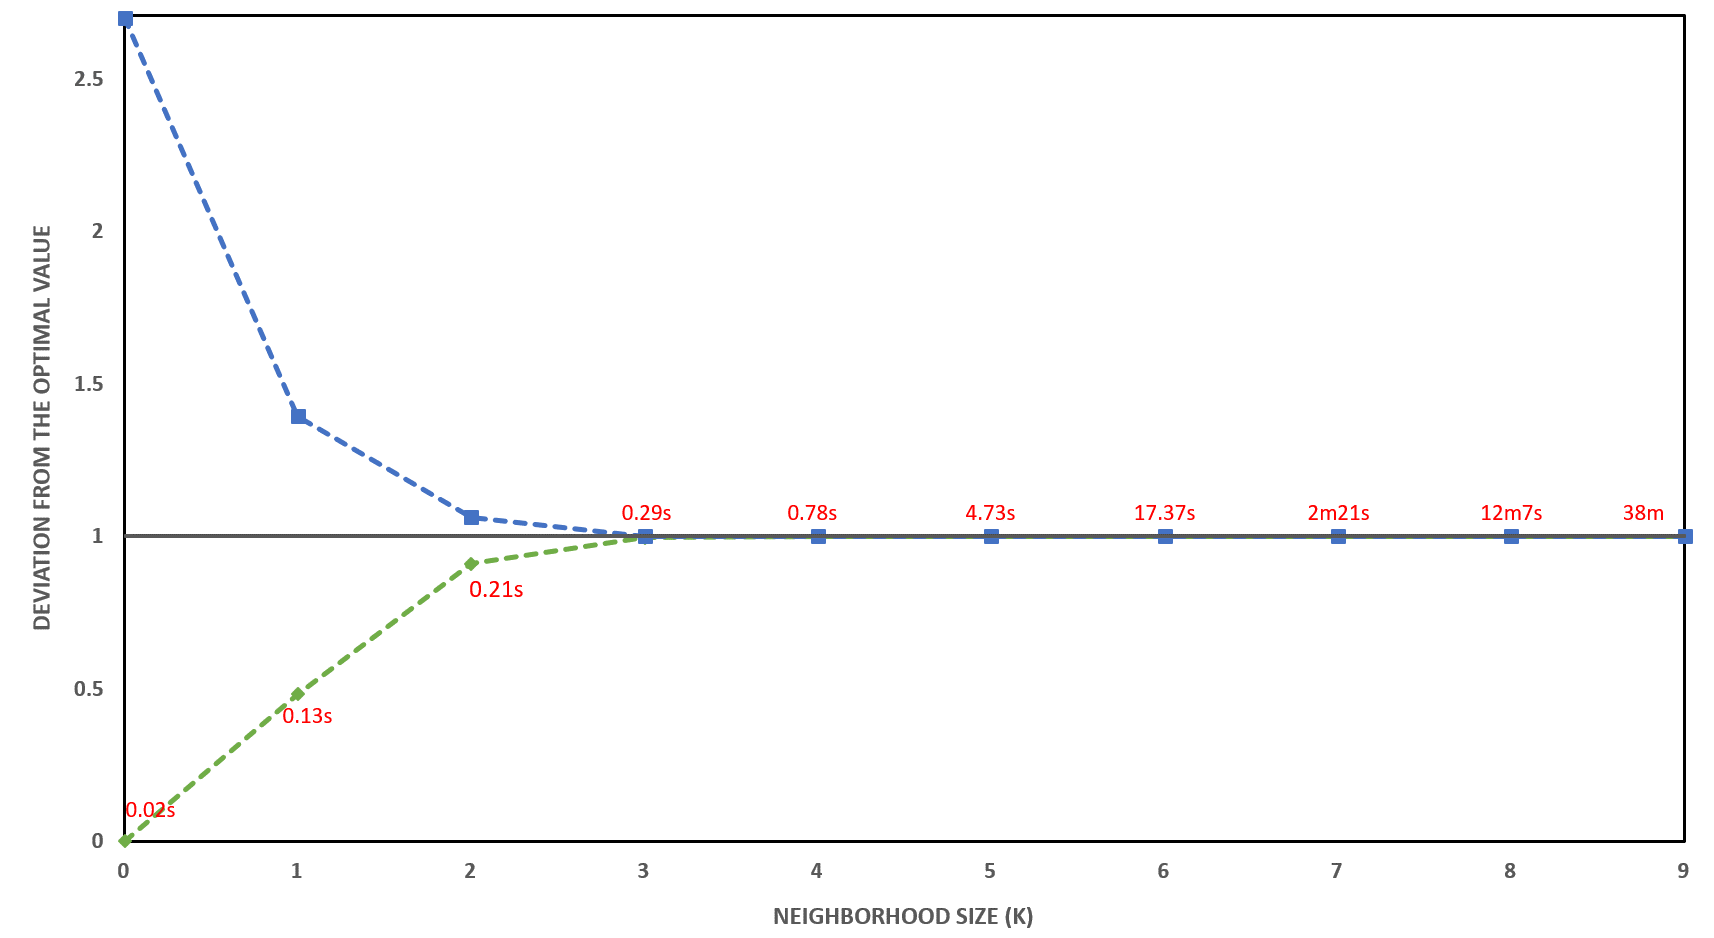
\includegraphics[width=\textwidth]{img/result_DNEG_n15k4.PNG}
	\caption{The average results for $n=10, r=4$.}
	\label{fig:n10k1j4}
\end{figure}
\begin{figure}
	\centering
	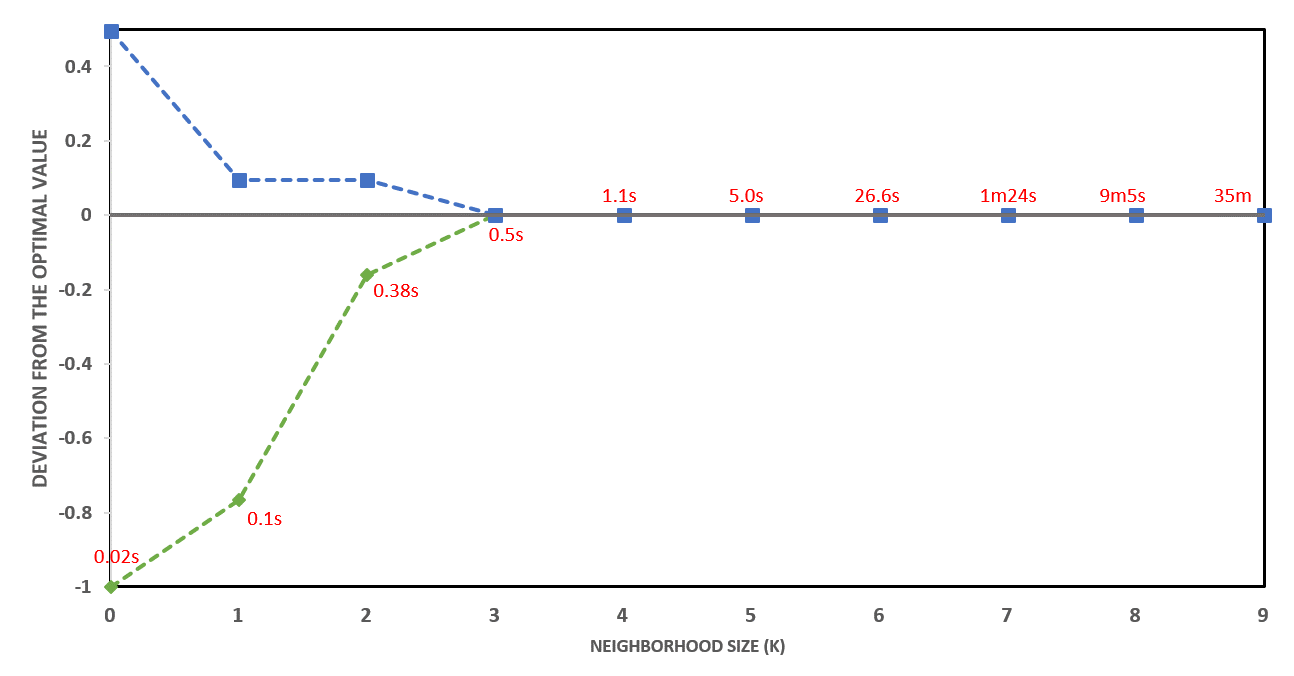
\includegraphics[width=\textwidth]{img/result_DNEG_n15k4j0.PNG}
	\caption{The results for $n=15, r=4$.}
	\label{fig:n15k4j0}
\end{figure}



Table \ref{tab:knapsack_interdict1} and Table \ref{tab:knapsack_interdict2} report the average performance of CCLW, Mibs, and $k=1,2,3$ for extended formulations. For the CCLW  algorithm, the bilevel linear programming relaxation is used to obtain valid upper bound.  The average number of runtime (in seconds) are also reported. For the solver Mibs, we report the average runtime for the instances that can be solved within the time limit 10 mins. For the instances that are not able to be solved within 10 mins, we report ratios of between the best lower bound and the optimal value as the column ``ObjL''. Also, the ratio between the best upper bound and the optimal value is reported as the column ``ObjU''. For the bilevel k-optimality problem, the BP$_k$ provides a valid lower bound and a feasible leader's decision $x^*_k$. We report the ration between the optimal value of BP$_k$ and the primal problem in the column ``ObjL''. Meantime, we can solve the follower's problem with respect to $x^*_k$ to obtain a valid upper bound for the bilevel interdiction problem, whose ration with the optimal value of the primal problem is also reported in the column ``ObjU''.

From Table \ref{tab:knapsack_interdict1}-\ref{tab:knapsack_interdict2}, we have the following observations:
%\begin{itemize}
%%	\item CCLW vs DNeg. When $r < 5$, DNeg algorithm performs better, as it runs less iterations. On the other hand, when $r > 5$, CCLW can find a very good upper bound that is close to the optimal value. Thus, it only needs less than 2 iterations to solve the problem.
%%	\item DNeg$_1$ vs DNeg. In general DNeg$_1$ algorithm needs less iterations than DNeg. However, if the iterations become large, the master problem in DNeg$_1$ is harder to solve, which would increase the runtime. On the other hand, $BP_1$ can provide a very tight lower bound and upper bound when $r \geq 5$, so that DNeg$_1$ algorithm can converge quickly within 2 iterations.
%%	\item CCLW vs DNeg$_1$. With the decrease of $k$, the quality of upper bounds in CCLW and $BP_1$ will fall off. It might be due to the fact that if $r$ is small, then the feasible solutions of the two decision-makers are restricted, which results in the large difference between relaxation and primal problem. Also, in general, CCLW can provide better upper bound than $BP_1$. However, the interesting question is how about $BP_2$ and $BP_3$?
%\end{itemize}


% Table generated by Excel2LaTeX from sheet 'Sheet4'
\begin{sidewaystable}[htbp]
	\centering
	\begin{adjustbox}{width=\columnwidth, height=0.3\textheight, center}
			\begin{tabular}{rrrrccccrrrrrrrrrrrrrrrrrrr}
			\toprule
			&       & \multicolumn{1}{c}{CCLW \cite{caprara2016bilevel}} &       & \multicolumn{4}{c}{Mibs \cite{tahernejad2016branch}}      &       & \multicolumn{3}{c}{Single-level relaxation ($k=0$)} &       & \multicolumn{4}{c}{$k=1$}       &       & \multicolumn{3}{c}{$k=2$} &       &       & \multicolumn{4}{c}{$k=3$} \\
			\cmidrule{3-3}\cmidrule{5-8}\cmidrule{10-12}\cmidrule{14-17}\cmidrule{19-22}\cmidrule{24-27}    \multicolumn{1}{c}{$n$} & \multicolumn{1}{c}{$r$} & \multicolumn{1}{c}{Time} &       & Unsolved & ObjL  & ObjU  & Time  &       & \multicolumn{1}{c}{ObjL} & \multicolumn{1}{c}{ObjU} & \multicolumn{1}{c}{Time} &       & \multicolumn{1}{c}{ObjL} & \multicolumn{1}{c}{ObjU} & \multicolumn{1}{c}{Time} & \multicolumn{1}{c}{Ext Time} &       & \multicolumn{1}{c}{ObjL} & \multicolumn{1}{c}{ObjU} & \multicolumn{1}{c}{Time} & \multicolumn{1}{c}{Ext Time} &       & \multicolumn{1}{c}{ObjL} & \multicolumn{1}{c}{ObjU} & \multicolumn{1}{c}{Time} & \multicolumn{1}{c}{Ext Time} \\
			\midrule
			10    & 0     & 0.13  &       &       &       &       & 0.01  &       & 0     & 1.8   & 0.02  &       & 0.34  & 1.8   & 0.04  & 0.14  &       & 0.99  & 1.01  & 0.02  & 0.03  &       & 1     & 1     & 0.03  & 0.03 \\
			10    & 1     & 0.17  &       &       &       &       & 0.02  &       & 0     & 1.8   & 0.01  &       & 0.23  & 1.41  & 0.04  & 0.07  &       & 0.78  & 1.17  & 0.07  & 0.05  &       & 0.99  & 1     & 0.06  & 0.09 \\
			10    & 2     & 0.26  &       &       &       &       & 0.03  &       & 0     & 1.93  & 0.01  &       & 0.41  & 1.47  & 0.04  & 0.08  &       & 0.94  & 1.11  & 0.14  & 0.12  &       & 1     & 1     & 0.19  & 0.23 \\
			10    & 3     & 0.37  &       &       &       &       & 0.05  &       & 0     & 2.73  & 0.01  &       & 0.34  & 1.36  & 0.05  & 0.06  &       & 0.94  & 1.05  & 0.13  & 0.1   &       & 1     & 1.01  & 0.19  & 0.17 \\
			10    & 4     & 0.33  &       &       &       &       & 0.03  &       & 0     & 12.09 & 0.02  &       & 0.52  & 1.51  & 0.08  & 0.1   &       & 0.98  & 1.12  & 0.11  & 0.08  &       & 1.03  & 1.03  & 0.14  & 0.15 \\
			\midrule
			20    & 0     & 0.15  &       &       &       &       & 0.14  &       & 0     & 1.59  & 0.01  &       & 0.14  & 1.43  & 0.08  & 0.07  &       & 0.75  & 1.12  & 0.12  & 0.09  &       & 0.97  & 1     & 0.19  & 0.13 \\
			20    & 1     & 1.26  &       &       &       &       & 1.91  &       & 0     & 1.8   & 0.01  &       & 0.14  & 1.3   & 0.07  & 0.1   &       & 0.71  & 1.15  & 0.13  & 0.15  &       & 0.99  & 1.03  & 0.23  & 0.23 \\
			20    & 2     & 2.15  &       &       &       &       & 9.7   &       & 0     & 1.98  & 0.01  &       & 0.19  & 1.37  & 0.12  & 0.09  &       & 0.78  & 1.11  & 0.18  & 0.16  &       & 0.98  & 1.03  & 0.33  & 0.25 \\
			20    & 3     & 0.93  &       &       &       &       & 15.12 &       & 0     & 2.62  & 0.01  &       & 0.34  & 1.7   & 0.15  & 0.09  &       & 0.84  & 1.13  & 0.15  & 0.15  &       & 1     & 1.01  & 0.25  & 0.2 \\
			20    & 4     & 0.97  &       &       &       &       & 7.9   &       & 0     & 3.45  & 0.01  &       & 0.63  & 1.43  & 0.11  & 0.1   &       & 0.89  & 1.03  & 0.16  & 0.15  &       & 1     & 1.01  & 0.23  & 0.2 \\
			\midrule
			30    & 0     & 1     &       &       &       &       & 2.98  &       & 0     & 1.54  & 0.01  &       & 0.06  & 1.38  & 0.1   & 0.07  &       & 0.7   & 1.12  & 0.18  & 0.2   &       & 1     & 1.01  & 0.42  & 0.35 \\
			30    & 1     & 8.17  &       & 6     & 0.95  & 1     & 212.99  &       & 0     & 1.82  & 0.01  &       & 0.1   & 1.45  & 0.11  & 0.08  &       & 0.73  & 1.13  & 0.22  & 0.15  &       & 0.97  & 1.01  & 1.01  & 0.92 \\
			30    & 2     & 19.99 &       & 8     & 0.81  & 1     & 249.20  &       & 0     & 1.94  & 0.01  &       & 0.19  & 1.46  & 0.17  & 0.09  &       & 0.73  & 1.09  & 0.19  & 0.16  &       & 0.97  & 1.02  & 1.29  & 0.89 \\
			30    & 3     & 15.46 &       & 10    & 0.81  & 1.03  &       &       & 0     & 2.54  & 0.01  &       & 0.31  & 1.62  & 0.16  & 0.12  &       & 0.8   & 1.16  & 0.27  & 0.21  &       & 0.99  & 1.01  & 1.16  & 0.64 \\
			30    & 4     & 0.33  &       & 5     & 0.82  & 1     & 203.42  &       & 0     & 3.82  & 0.01  &       & 0.67  & 1.52  & 0.18  & 0.16  &       & 1     & 1.03  & 0.28  & 0.21  &       & 1.01  & 1.01  & 0.62  & 0.38 \\
			\midrule
			40    & 0     & 2.21  &       & 2     & 0.86  & 1.00  & 73.03  &       & 0     & 1.66  & 0.01  &       & 0.07  & 1.35  & 0.09  & 0.07  &       & 0.57  & 1.21  & 0.24  & 0.19  &       & 1     & 1.05  & 2.22  & 1.52 \\
			40    & 1     & 27.7  &       & 10    & 0.70  & 1     &       &       & 0     & 1.8   & 0.01  &       & 0.11  & 1.46  & 0.14  & 0.09  &       & 0.65  & 1.12  & 0.27  & 0.24  &       & 0.96  & 1.03  & 3.84  & 2.81 \\
			40    & 2     & 378.93 &       & 10    & 0.57  & 1     &       &       & 0     & 2     & 0.01  &       & 0.2   & 1.4   & 0.19  & 0.09  &       & 0.69  & 1.11  & 0.39  & 0.32  &       & 0.97  & 1.02  & 5.28  & 3.14 \\
			40    & 3     & 82.22 &       & 10    & 0.54  & 1.00  &       &       & 0     & 2.5   & 0.01  &       & 0.34  & 1.48  & 0.21  & 0.13  &       & 0.82  & 1.17  & 0.56  & 0.33  &       & 0.99  & 1     & 5.63  & 2.64 \\
			40    & 4     & 78.1  &       & 10    & 0.60  & 1     &       &       & 0     & 3.22  & 0.01  &       & 0.62  & 1.49  & 0.21  & 0.16  &       & 0.92  & 1.08  & 0.47  & 0.24  &       & 1     & 1     & 3.01  & 1.78 \\
			\midrule
			50    & 0     & 6.51  &       & 6     & 0.86  & 1     & 166.22  &       & 0     & 1.66  & 0.01  &       & 0.06  & 1.45  & 0.08  & 0.09  &       & 0.6   & 1.29  & 0.39  & 0.29  &       & 1.04  & 1.07  & 10.41 & 8.78 \\
			50    & 1     & 632.64 &       & 10    & 0.69  & 1     &       &       & 0     & 1.79  & 0.01  &       & 0.09  & 1.42  & 0.15  & 0.1   &       & 0.69  & 1.09  & 0.64  & 0.46  &       & 0.98  & 1.01  & 21.81 & 10.44 \\
			50    & 2     & 1422.86 &       & 10    & 0.49  & 1     &       &       & 0     & 2.05  & 0.01  &       & 0.18  & 1.42  & 0.23  & 0.09  &       & 0.64  & 1.07  & 0.64  & 0.45  &       & 0.98  & 1.01  & 22.14 & 11.69 \\
			50    & 3     & 1312.54 &       & 10    & 0.41  & 1.03  &       &       & 0     & 2.61  & 0.01  &       & 0.37  & 1.49  & 0.25  & 0.16  &       & 0.79  & 1.16  & 0.84  & 0.52  &       & 0.99  & 1.01  & 13.3  & 8.39 \\
			50    & 4     & 10.28 &       & 10    & 0.46  & 1.01  &       &       & 0     & 3.35  & 0.02  &       & 0.65  & 1.52  & 0.31  & 0.21  &       & 0.93  & 1.06  & 0.9   & 0.48  &       & 1     & 1     & 7.75  & 3.97 \\
			\bottomrule
		\end{tabular}%
	\end{adjustbox}

	\caption{Results of hard instances for knapsack interdiction problem.}
	
	\label{tab:knapsack_interdict1}%
\end{sidewaystable}%

% Table generated by Excel2LaTeX from sheet 'Sheet4'
\begin{sidewaystable}[htbp]
	\begin{adjustbox}{width=\columnwidth, height=0.3\textheight, center}
		\begin{tabular}{rrrrccccrrrrrrrrrrrrrrrrrrr}
			\toprule
			&       & \multicolumn{1}{c}{CCLW \cite{caprara2016bilevel}} &       & \multicolumn{4}{c}{Mibs \cite{tahernejad2016branch}}      &       & \multicolumn{3}{c}{Single-level relaxation ($k=0$)} &       & \multicolumn{4}{c}{$k=1$}       &       & \multicolumn{3}{c}{$k=2$} &       &       & \multicolumn{4}{c}{$k=3$} \\
			\cmidrule{3-3}\cmidrule{5-8}\cmidrule{10-12}\cmidrule{14-17}\cmidrule{19-22}\cmidrule{24-27}    \multicolumn{1}{c}{$n$} & \multicolumn{1}{c}{$r$} & \multicolumn{1}{c}{Time} &       & Unsolved & ObjL  & ObjU  & Time  &       & \multicolumn{1}{c}{ObjL} & \multicolumn{1}{c}{ObjU} & \multicolumn{1}{c}{Time} &       & \multicolumn{1}{c}{ObjL} & \multicolumn{1}{c}{ObjU} & \multicolumn{1}{c}{Time} & \multicolumn{1}{c}{Ext Time} &       & \multicolumn{1}{c}{ObjL} & \multicolumn{1}{c}{ObjU} & \multicolumn{1}{c}{Time} & \multicolumn{1}{c}{Ext Time} &       & \multicolumn{1}{c}{ObjL} & \multicolumn{1}{c}{ObjU} & \multicolumn{1}{c}{Time} & \multicolumn{1}{c}{Ext Time} \\
			\midrule
			10    & 5     & 0.09  &       &       &       &       & 0.02  &       & 0     & 11.14 & 0.01  &       & 0.72  & 1.94  & 0.05  & 0.06  &       & 1     & 1     & 0.08  & 0.09  &       & 1     & 1     & 0.07  & 0.12 \\
			10    & 6     & 0.09  &       &       &       &       & 0.02  &       & 0     & 10.6  & 0.01  &       & 0.93  & 1.05  & 0.07  & 0.04  &       & 1     & 1     & 0.06  & 0.06  &       & 1     & 1     & 0.08  & 0.15 \\
			10    & 7     & 0.03  &       &       &       &       & 0.02  &       & 0     & 9.61  & 0.01  &       & 1     & 1     & 0.05  & 0.06  &       & 1     & 1     & 0.08  & 0.07  &       & 1     & 1     & 0.08  & 0.08 \\
			10    & 8     & 0.03  &       &       &       &       & 0.01  &       & 0     & 18.88 & 0.01  &       & 1     & 1     & 0.07  & 0.06  &       & 1     & 1     & 0.07  & 0.05  &       & 1     & 1     & 0.07  & 0.04 \\
			10    & 9     & 0.03  &       &       &       &       & 0.01  &       & 0     & 49.58 & 0.01  &       & 1     & 1     & 0.09  & 0.05  &       & 1     & 1     & 0.05  & 0.04  &       & 1     & 1     & 0.05  & 0.07 \\
			\midrule
			20    & 5     & 0.07  &       &       &       &       & 2.02  &       & 0     & 5.87  & 0.01  &       & 0.97  & 1.15  & 0.11  & 0.09  &       & 1     & 1     & 0.16  & 0.13  &       & 1     & 1     & 0.19  & 0.18 \\
			20    & 6     & 0.05  &       &       &       &       & 0.98  &       & 0     & 10.24 & 0.01  &       & 0.99  & 1.06  & 0.11  & 0.13  &       & 1     & 1     & 0.18  & 0.09  &       & 1     & 1     & 0.16  & 0.16 \\
			20    & 7     & 0.06  &       &       &       &       & 0.32  &       & 0     & 32.24 & 0.01  &       & 1     & 1     & 0.11  & 0.1   &       & 1     & 1     & 0.09  & 0.09  &       & 1     & 1     & 0.14  & 0.16 \\
			20    & 8     & 0.04  &       &       &       &       & 0.04  &       & 0     & 92.07 & 0.01  &       & 1     & 1     & 0.08  & 0.09  &       & 1     & 1     & 0.08  & 0.08  &       & 1     & 1     & 0.11  & 0.13 \\
			20    & 9     & 0.03  &       &       &       &       & 0.02  &       & 0     & 257   & 0.01  &       & 1     & 1     & 0.06  & 0.04  &       & 1     & 1     & 0.05  & 0.07  &       & 1     & 1     & 0.07  & 0.1 \\
			\midrule
			30    & 5     & 0.08  &       & 2     & 0.97  & 1     & 203.42  &       & 0     & 6.44  & 0.01  &       & 0.99  & 1.23  & 0.21  & 0.11  &       & 1     & 1     & 0.21  & 0.21  &       & 1     & 1     & 0.45  & 0.27 \\
			30    & 6     & 0.05  &       &       &       &       & 19.62  &       & 0     & 9.09  & 0.01  &       & 0.99  & 1.08  & 0.19  & 0.13  &       & 1     & 1     & 0.25  & 0.14  &       & 1     & 1     & 0.29  & 0.25 \\
			30    & 7     & 0.06  &       &       &       &       & 3.19  &       & 0     & 35.47 & 0.01  &       & 1     & 1     & 0.17  & 0.07  &       & 1     & 1     & 0.17  & 0.1   &       & 1     & 1     & 0.22  & 0.22 \\
			30    & 8     & 0.03  &       &       &       &       & 0.24  &       & 0     & 88.24 & 0.01  &       & 1     & 1     & 0.1   & 0.08  &       & 1     & 1     & 0.07  & 0.1   &       & 1     & 1     & 0.14  & 0.15 \\
			30    & 9     & 0.08  &       &       &       &       & 0.02  &       & 0     & 239.54 & 0.01  &       & 1     & 1     & 0.07  & 0.07  &       & 1     & 1     & 0.06  & 0.07  &       & 1     & 1     & 0.16  & 0.15 \\
			\midrule
			40    & 5     & 0.15  &       & 9     & 0.75  & 1.03  & 24.52  &       & 0     & 5.36  & 0.01  &       & 0.99  & 1.19  & 0.29  & 0.14  &       & 1.02  & 1.02  & 0.27  & 0.19  &       & 1.02  & 1.02  & 1.4   & 0.82 \\
			40    & 6     & 0.05  &       & 1     & 0.83  & 1     & 62.85  &       & 0     & 14.73 & 0.01  &       & 1     & 1     & 0.21  & 0.12  &       & 1     & 1     & 0.22  & 0.16  &       & 1     & 1     & 0.46  & 0.61 \\
			40    & 7     & 0.07  &       & 2     & 0.91  & 1     & 11.29  &       & 0     & 21.12 & 0.01  &       & 1     & 1     & 0.21  & 0.15  &       & 1     & 1     & 0.18  & 0.13  &       & 1     & 1     & 0.3   & 0.6 \\
			40    & 8     & 0.06  &       &       &       &       & 2.33  &       & 0     & 35.59 & 0.01  &       & 1     & 1     & 0.13  & 0.1   &       & 1     & 1     & 0.1   & 0.09  &       & 1     & 1     & 0.21  & 0.47 \\
			40    & 9     & 0.06  &       &       &       &       & 0.20  &       & 0     & 324.56 & 0.01  &       & 1     & 1     & 0.08  & 0.06  &       & 1     & 1     & 0.05  & 0.09  &       & 1     & 1     & 0.12  & 0.32 \\
			\midrule
			50    & 5     & 0.37  &       & 10    & 0.58  & 1.01  &       &       & 0     & 5.43  & 0.01  &       & 0.97  & 1.07  & 0.59  & 0.19  &       & 1     & 1     & 0.68  & 0.25  &       & 1     & 1     & 3.37  & 1.98 \\
			50    & 6     & 0.07  &       & 8     & 0.72  & 1.01  & 326.93  &       & 0     & 11.86 & 0.02  &       & 1     & 1     & 0.41  & 0.18  &       & 1     & 1     & 0.31  & 0.21  &       & 1     & 1     & 1.34  & 1.77 \\
			50    & 7     & 0.15  &       & 5     & 0.94  & 1     & 164.01  &       & 0     & 17.11 & 0.01  &       & 1     & 1     & 0.26  & 0.13  &       & 1     & 1     & 0.22  & 0.21  &       & 1     & 1     & 0.65  & 1.4 \\
			50    & 8     & 0.05  &       &       &       &       & 5.96  &       & 0     & 86.23 & 0.02  &       & 1     & 1     & 0.2   & 0.08  &       & 1     & 1     & 0.15  & 0.24  &       & 1     & 1     & 0.45  & 0.57 \\
			50    & 9     & 0.04  &       &       &       &       & 0.07  &       & 0     & 90.79 & 0.01  &       & 1     & 1     & 0.06  & 0.16  &       & 1     & 1     & 0.14  & 0.11  &       & 1     & 1     & 0.21  & 0.41 \\
			\bottomrule
		\end{tabular}%
	\end{adjustbox}
	\caption{Results of easy instances for knapsack interdiction problem.}
	\label{tab:knapsack_interdict2}%
\end{sidewaystable}%






% Table generated by Excel2LaTeX from sheet 'Sheet1'
%\begin{table}[t]
%	\centering
%	\begin{tabular}{ccccccccccccc}
%		\toprule
%		&       & \multicolumn{3}{c}{CCLW \cite{caprara2016bilevel}} &       & \multicolumn{4}{c}{DNeg$_1$}   &       & \multicolumn{2}{c}{DNeg} \\
%		\cmidrule{3-5}\cmidrule{7-10}\cmidrule{12-13}    n     & r     & ObjU  & Iters & Time  &       & ObjL  & ObjU  & Iters & Time  &       & Iters & Time \\ \hline
%		\multirow{10}[1]{*}{15} & 1     & 1.6   & 1.3   & 0.07  &       & 0.34  & 1.67  & 1.5   & 0.13  &       & 1.5   & 0.04 \\
%		& 2     & 1.24  & 2.8   & 0.13  &       & 0.23  & 1.22  & 3     & 0.21  &       & 3.1   & 0.15 \\
%		& 3     & 1.19  & 4.4   & 0.41  &       & 0.41  & 1.2   & 4.3   & 0.51  &       & 4.7   & 0.25 \\
%		& 4     & 1.06  & 5.5   & 0.38  &       & 0.34  & 1.24  & 7.5   & 0.91  &       & 8.3   & 0.67 \\
%		& 5     & 1.05  & 3.8   & 0.34  &       & 0.52  & 1.42  & 6.3   & 1.03  &       & 8     & 0.5 \\
%		& 6     & 1     & 1.6   & 0.1   &       & 1     & 1     & 2.9   & 0.33  &       & 7.1   & 0.47 \\
%		& 7     & 1     & 1.5   & 0.15  &       & 1     & 1     & 2     & 0.64  &       & 8.2   & 0.55 \\
%		& 8     & 1     & 1     & 0.03  &       & 1     & 1     & 1     & 0.06  &       & 8.7   & 0.97 \\
%		& 9     & 1     & 1     & 0.03  &       & 1     & 1     & 1     & 0.08  &       & 6.2   & 0.23 \\
%		& 10    & 1     & 1     & 0.03  &       & 1     & 1     & 1     & 0.05  &       & 6.9   & 0.85 \\
%		\midrule
%		\multirow{10}[2]{*}{25} & 1     & 1.1   & 2.4   & 0.23  &       & 0.14  & 1.14  & 3.2   & 0.68  &       & 3.3   & 0.37 \\
%		& 2     & 1.05  & 211.9 & 25.8  &       & 0.14  & 1.08  & 15.7  & 3.85  &       & 16.5  & 3.12 \\
%		& 3     & 1.04  & 22.8  & 4.72  &       & 0.19  & 1.23  & 30.7  & 8.51  &       & 32.1  & 5.21 \\
%		& 4     & 1.03  & 208.1 & 21.73 &       & 0.34  & 1.38  & 45.3  & 13.4  &       & 47    & 6.8 \\
%		& 5     & 1.03  & 10.2  & 1.65  &       & 0.63  & 1.25  & 37.4  & 19.79 &       & 48    & 8.37 \\
%		& 6     & 1     & 1     & 0.12  &       & 0.97  & 1.17  & 2.6   & 0.8   &       & 61.6  & 10.54 \\
%		& 7     & 1     & 1     & 0.06  &       & 0.99  & 1.05  & 1.4   & 0.15  &       & 33.9  & 6.69 \\
%		& 8     & 1     & 1     & 0.1   &       & 1     & 1     & 1     & 0.08  &       & 55    & 19.21 \\
%		& 9     & 1     & 1     & 0.04  &       & 1     & 1     & 1     & 0.08  &       & 23.8  & 3.14 \\
%		& 10    & 1     & 1     & 0.03  &       & 1     & 1     & 1     & 0.04  &       & 13    & 1.75 \\
%		\midrule
%		\multirow{10}[1]{*}{30} & 1     & 1.07  & 6.3   & 0.86  &       & 0.09  & 1.1   & 7     & 1.88  &       & 7.2   & 1.37 \\
%		& 2     & 1.05  & 224.7 & 32.54 &       & 0.13  & 1.15  & 29.5  & 8.6   &       & 29.2  & 6.16 \\
%		& 3     & 1.04  & 50.9  & 11.35 &       & 0.17  & 1.18  & 61.3  & 22.96 &       & 62.6  & 12.68 \\
%		& 4     & 1.01  & 426.4 & 73.08 &       & 0.3   & 1.42  & 168.7 & 144.44 &       & 174.9 & 79.33 \\
%		& 5     & 1.01  & 206.5 & 21.44 &       & 0.55  & 1.44  & 132.5 & 126.14 &       & 163.4 & 60.54 \\
%		& 6     & 1     & 1     & 0.15  &       & 0.9   & 1.24  & 21.2  & 23.9  &       & 141.9 & 59.46 \\
%		& 7     & 1     & 1     & 0.07  &       & 0.99  & 1.06  & 1.2   & 0.15  &       & 126.4 & 50.22 \\
%		& 8     & 1     & 1     & 0.04  &       & 1     & 1     & 1     & 0.09  &       & 44.8  & 10.3 \\
%		& 9     & 1     & 1     & 0.04  &       & 1     & 1     & 1     & 0.11  &       & 40.9  & 8.31 \\
%		& 10    & 1     & 1     & 0.03  &       & 1     & 1     & 1     & 0.07  &       & 25.9  & 3.13 \\ \hline
%	\end{tabular}%
%	\caption{Results for knapsack interdiction problem.}
%	\label{tab:knapsack_interdict}%
%\end{table}%


\newpage
\section{Case study}
\subsection{vertex cover}
Given a graph $G = (N, E)$, the vertex cover problem is to find a subset of vertices whose total weight is as small as possible such that each vertex in the graph is either in this subset or connected to at least one vertex in this subset. There have three possible versions about bilevel vertex cover problem. The first version is that the leader destroys the vertices and then the follower finishes the vertex cover problem \cite{bazgan2011most}. Also, we assume that the weights of two decision-makers are different.

\begin{subequations}
	\begin{align}
	\text{[BVC]~}\max_x\; & \sum_j w_j^1 y_j \nonumber\\
	\text{s.t.~} & \sum_{j} x_j \leq b, \label{eq:BVC_1} \\
	& x_j \in \{0,1\} \quad \forall j\in N, \\
	& \min_y\;  \sum_j w_j^2 y_j \nonumber\\
	&\text{s.t.~}  x_j + y_j \leq 1 \quad \forall j\in N, \\
	& \quad \sum_{j\in N_i} y_j \geq 1 \quad \forall i\in N, \label{eq:BVC_3}\\
	& \quad y_j \in \{0, 1\} \quad \forall i \in N, \label{eq:BVC_4}
	\end{align}
\end{subequations}
where $N_j$ is the neighborhood of vertex $j\in N$, that includes $j$ itself. Let $\T^k = \{ (T_1, T_2): w^2(T_1) < w^2(T_2), |T_1\cup T_2|\leq k, T_1\cap T_2 = \emptyset, T_i \subseteq N\; i=1,2\}.$ To formulate the corresponding bilevel k-optimality problem, we introduce logistic variables $z_{i,t}\in \{0, 1\}$ for $i\in N, t\in \T^k$. 
\begin{subequations}
	\begin{align}
	[\text{BVC}_k]\;\max_x\; & \sum_j w_j^1 y_j \nonumber\\
	\text{s.t.~} & \eqref{eq:BVC_1} - \eqref{eq:BVC_4}, \nonumber\\
	& \sum_{j\in N_i} y_j + (h_{i, t} - \mu_i) z_{i, t} \leq h_{i, t} \quad \forall i\in N, t\in \T^k \\
	& \sum_{i=1}^n z_{i, t} - \sum_{j\in T_2} (1 - y_j + x_j) - \sum_{j\in T_1} (x_j + y_j) \leq n-1 \forall t = (T_1, T_2) \in \T^k, \label{eq:BVC_k_1}\\
	&  z_{i, t} \in \{0, 1\} \;\forall i\in N, t\in \T^k,
	\end{align}
\end{subequations}
where $h_{i, t} = |N_i \cap T_2| - |N_i \cap T_1|$ for $t = (T_1, T_2) \in \T^k$, and $\mu_i = |N_i|$ for all $i\in N$. We next discuss how to reduce the size $\T^k$ and the formulation  size.

\noindent\textbf{Preprocessing.}
\begin{itemize}
	\item For any $t=(T_1, T_2) \in \T^k$, if there exists $i \in N$ such that either $N_i \subseteq T_1$ or $N_i \subseteq T_2$, then we can remove $t$ from $\T^k.$
	\item If $|N_i \cap T_1| - |N_i \cap T_2| \geq 0$ for some $i\in N$ and $t = (T_1, T_2)\in \T^k$, i.e., $h_{i, t} \leq 0$, then we can set $z_{i, t} = 1$.
	\item For any $t = (T_1, T_2) \in T^k$, then we can remove  $(T_1, T')$ in $\T^k$ such that $T_2 \subseteq T'$.
	\item If $h_{i, t_1} = h_{i, t_2}$ for some $t_1, t_2 \in \T^k$, then we set $z_{i, t_1} = z_{i, t_2}$.
\end{itemize}

\noindent \textbf{Extended formulation.} For each $i\in [n]$, we sort $h_{i, t}$ into a decreasing order such that $h_{i, (1)} \leq h_{i, (2)} \leq \cdots \leq h_{i, (\ell)}$, where $\ell = |\T^k|$. Then the extended formulation for BVC is formalized as
\begin{subequations}
	\begin{align}
	[\text{EBVC}_k]\;\max_x\; & \sum_j w_j^1 y_j \nonumber\\
	\text{s.t.~} & \eqref{eq:BVC_1} - \eqref{eq:BVC_4}, \eqref{eq:BVC_k_1}, \nonumber\\
	& \sum_{j\in N_i} y_j + \sum_{t=1}^\ell (h_{i, (t)} - h_{i, (t+1)}) v_{i, (t)} \leq h_{i, (1)} \quad \forall i\in N, \\
	& v_{i, (t)} \geq v_{i, (t+1)} \quad \forall i\in N, t\in \T^k, \\
	& v_{i, (t)} \leq z_{i, (t)} \quad \forall i\in N, t\in \T^k,\\ 
	&  z_{i, t} \in \{0, 1\}, v_{i, t}\in \{0, 1\} \;\forall i\in N, t\in \T^k, \nonumber
	\end{align}
\end{subequations}
where $h_{i, (\ell+1)} = \mu_i$ for $i\in N$.

\subsection{Experiment}
\textbf{Test Setup.} We randomly generate graphs through SNAP \cite{leskovec2016snap}, in which the degree of each node is no less than $5, 8, 10, 12, 15$ with respect to node size $10, 20, 30, 40, 50.$  We examine the performances by comparing the results of Mibs \cite{denegre2011interdiction}. We set time limit for Mibs for 30 mins to avoid out of memory.

For each class of $n$, we generate 10 instances and report their average performance. The bilevel feasible solution obtained through Mibs within 30 min (i.e., the lower bound) is used as the baseline. We report the solving time and the ratio between upper bound and lower bound for solver Mibs. As for the bilevel program with $k$ optimality, the ratios between the obtained upper bound and the lower bound from Mibs are shown as the column ``ObjU''. we report the ratios between the best lower bound and the lower bound obtained through Mibs as the column ``ObjL''. The runtime to solve BP$_k$ and EBP$_k$ are reported in columns ``Time'' and ``Ext Time'', respectively.


% Table generated by Excel2LaTeX from sheet 'interdiction'
\begin{table}[htbp]
	\centering
	
	\begin{adjustbox}{width=\columnwidth, height=0.15\textheight,  center}
			% Table generated by Excel2LaTeX from sheet 'interdiction'
		\begin{tabular}{ccccccccccccccccccccccccc}
			\toprule
			&       &       &       & \multicolumn{2}{c}{Mibs} &       & \multicolumn{3}{c}{$k=0$} &       & \multicolumn{4}{c}{$k=1$}       &       & \multicolumn{4}{c}{$k=2$}       &       & \multicolumn{4}{c}{$k=3$} \\
			\cmidrule{5-6}\cmidrule{8-10}\cmidrule{12-15}\cmidrule{17-20}\cmidrule{22-25}    $n$     & deg   & $b$     &       & ObjU  & Time  &       & ObjU  & ObjL  & Time  &       & ObjU  & ObjL  & Time  & Ext Time &       & ObjU  & ObjL  & Time  & Ext Time &       & ObjU  & ObjL  & Time  & Ext Time \\
			\midrule
			\multicolumn{25}{c}{Symmetric Objective} \\
			\midrule
			10    & 5     & 5     &       & 1     & 0.57  &       & 4     & 0.27  & 0.02  &       & 1.38  & 0.27  & 0.14  & 0.13  &       & 1.06  & 0.87  & 0.14  & 0.14  &       & 1.03  & 0.95  & 0.17  & 0.2 \\
			20    & 8     & 8     &       & 1     & 457.74 &       & 6.46  & 0.19  & 0.01  &       & 1.94  & 0.19  & 0.17  & 0.12  &       & 1.42  & 0.81  & 0.28  & 0.28  &       & 1.17  & 0.75  & 0.86  & 1.54 \\
			30    & 10    & 10    &       & 7.17  & 1800  &       & 8.58  & 0.2   & 0.01  &       & 2.56  & 0.2   & 0.21  & 0.22  &       & 1.8   & 0.69  & 2.2   & 2.73  &       & 1.48  & 0.81  & 26.06 & 57.8 \\
			40    & 12    & 12    &       & 12.11 & 1800  &       & 13.24 & 0.23  & 0.02  &       & 4.02  & 0.23  & 1.35  & 1.23  &       & 2.56  & 0.63  & 33.48 & 30.46 &       & 1.87  & 0.95  & 2609.58 & 3527.47 \\
			50    & 15    & 15    &       & 17.77 & 1800  &       & 18.63 & 0.26  & 0.02  &       & 4.99  & 0.26  & 4.86  & 4.28  &       & 3.27  & 0.63  & 396.2 & 418.66 &       & 1.94  & 1.1   & 3600 & 3600 \\
			\midrule
			\multicolumn{25}{c}{Asymmetric Objective} \\
			\midrule
			10    & 5     & 5     &       & 1     & 0.54  &       & 3.12  & 0.53  & 0.02  &       & 1.07  & 0.53  & 0.14  & 0.13  &       & 1.04  & 0.76  & 0.16  & 0.12  &       & 1     & 0.96  & 0.15  & 0.19 \\
			20    & 8     & 8     &       & 1     & 438.88 &       & 3.97  & 0.47  & 0.02  &       & 1.3   & 0.47  & 0.15  & 0.12  &       & 1.17  & 0.61  & 0.27  & 0.2   &       & 1.05  & 0.68  & 0.75  & 0.92 \\
			30    & 10    & 10    &       & 4.32  & 1800  &       & 5.17  & 0.48  & 0.02  &       & 1.61  & 0.48  & 0.22  & 0.21  &       & 1.4   & 0.65  & 1.24  & 0.98  &       & 1.26  & 0.75  & 10.07 & 20.84 \\
			40    & 12    & 12    &       & 5.38  & 1800  &       & 5.88  & 0.49  & 0.02  &       & 1.76  & 0.49  & 1.38  & 1.35  &       & 1.45  & 0.63  & 10.01 & 10.35 &       & 1.31  & 0.75  & 451.97 & 699.72 \\
			50    & 15    & 15    &       & 6.88  & 1800  &       & 7.26  & 0.6   & 0.02  &       & 1.88  & 0.63  & 6.52  & 5.47  &       & 1.64  & 0.83  & 58.4  & 59.5  &       & 1.45  & 0.96  & 3579.93 & 3446.93 \\
			\bottomrule☼
		\end{tabular}%
	\end{adjustbox}
	\caption{The performance of BP$_k$ on the bilevel vertex cover problem.}
	\label{tab:addlabel}%
\end{table}%



% Table generated by Excel2LaTeX from sheet 'n30b10deg'
\begin{sidewaystable}[htbp]
	\centering
	\caption{Add caption}
	\begin{adjustbox}{width=\columnwidth, height=0.2\textheight, center}
		\begin{tabular}{ccccccccccccccccccccc}
			\toprule
			&       &       &       & \multicolumn{2}{c}{k=0} &       & \multicolumn{4}{c}{K=1}       &       & \multicolumn{4}{c}{K=2}       &       & \multicolumn{4}{c}{K=3} \\
			\cmidrule{5-6}\cmidrule{8-11}\cmidrule{13-16}\cmidrule{18-21}    n     & deg   & b     &       & Gap   & Time  &       & GAP1 & GAP2 & Time  & Time ext &       & GAP1 & GAP2 & Time  & Time ext &       & GAP1 & GAP2 & Time  & Time ext \\
			\midrule
			30    & 10    & 10    &       & 0.91  & 0.02  &       & 0.69  & 0.7   & 0.31  & 0.27  &       & 0.73  & 0.54  & 1.42  & 1.12  &       & 0.75  & 0.4   & 10.04 & 20.77 \\
			30    & 11    & 10    &       & 0.89  & 0.02  &       & 0.72  & 0.59  & 0.3   & 0.24  &       & 0.75  & 0.57  & 1.27  & 1.17  &       & 0.77  & 0.5   & 9.44  & 17.3 \\
			30    & 12    & 10    &       & 0.9   & 0.02  &       & 0.74  & 0.62  & 0.24  & 0.22  &       & 0.76  & 0.52  & 0.94  & 0.92  &       & 0.78  & 0.48  & 7.74  & 15.9 \\
			30    & 13    & 10    &       & 0.91  & 0.01  &       & 0.75  & 0.62  & 0.26  & 0.23  &       & 0.78  & 0.48  & 1.09  & 0.94  &       & 0.8   & 0.35  & 7.27  & 14.9 \\
			30    & 14    & 10    &       & 0.91  & 0.02  &       & 0.76  & 0.6   & 0.27  & 0.2   &       & 0.78  & 0.53  & 0.88  & 0.82  &       & 0.79  & 0.31  & 5.89  & 11.56 \\
			30    & 15    & 10    &       & 0.91  & 0.02  &       & 0.78  & 0.6   & 0.24  & 0.21  &       & 0.8   & 0.46  & 0.8   & 0.72  &       & 0.82  & 0.32  & 5.62  & 12.69 \\
			30    & 16    & 10    &       & 0.93  & 0.02  &       & 0.79  & 0.66  & 0.2   & 0.16  &       & 0.81  & 0.56  & 0.59  & 0.55  &       & 0.82  & 0.31  & 4.43  & 9.82 \\
			30    & 17    & 10    &       & 0.93  & 0.02  &       & 0.8   & 0.64  & 0.21  & 0.19  &       & 0.81  & 0.6   & 0.46  & 0.48  &       & 0.83  & 0.2   & 4.01  & 8.01 \\
			30    & 18    & 10    &       & 0.93  & 0.02  &       & 0.82  & 0.61  & 0.23  & 0.17  &       & 0.83  & 0.57  & 0.39  & 0.36  &       & 0.83  & 0.37  & 3.45  & 8.36 \\
			30    & 19    & 10    &       & 0.93  & 0.02  &       & 0.83  & 0.61  & 0.21  & 0.18  &       & 0.83  & 0.44  & 0.29  & 0.34  &       & 0.85  & 0.12  & 2.91  & 6.47 \\
			30    & 20    & 10    &       & 0.93  & 0.02  &       & 0.84  & 0.58  & 0.23  & 0.17  &       & 0.85  & 0.48  & 0.28  & 0.23  &       & 0.86  & 0.26  & 2.42  & 5.35 \\
			\bottomrule
		\end{tabular}%
	\end{adjustbox}
	
	\label{tab:addlabel}%
	\footnote{``GAP1'' is computed by $(z_0^* - z_k^*) / z_0^*$}
	\footnote{``GAP2'' is computed by (ub - lb) / ub}
\end{sidewaystable}%


%The second version of bilevel vertex cover considers that two decision-makers construct a subset of vertices in the hierarchy sequence to satisfy the vertex cover properties. Two decision-makers have different weights on vertices.
%\begin{align*}
%\min_x\; & \sum_{i\in V_\ell} w_i^1 x_i + \sum_{i\in V_f} w_i^1 y_i\\
%\text{s.t.~} & \sum_{i} x_i \leq K, \\
%& x_i \in \{0,1\} \quad \forall i\in V_\ell, \\
%& \min_y\;  \sum_{i\in V_f} w_i^2 y_i \\
%&\text{s.t.~}  x_i + y_i \leq 1 \quad \forall i\in V, \\
%& \quad x_i + y_i + \sum_{j\in V_i} (x_j + y_j) \geq 1 \quad \forall i\in V,\\
%& \quad y_i \in \{0, 1\} \quad i\in V_f,
%\end{align*}
%where $V_\ell$ and $V_f$ are the subsets of vertices  controlled  by the leader and the follower, respectively.
%
%The third version considers the pricing problem \cite{baiou2016stackelberg}. The leader wishes to maximize his profit by setting the tolling in the vertex set. 
%\begin{align*}
%\max_x\; & \sum_i w_i x_i y_i\\
%\text{s.t.~} & \sum_{i} a_i x_i \leq K, \\
%& x_i \in \RR \quad \forall i\in V, \\
%& \min_y\;  \sum_i (c_i + w_ix_i) y_i \\
%& \text{s.t.~}  y_i + \sum_{j\in V_i} y_j \geq 1 \quad \forall i\in V,\\
%& \quad y_i \in \{0, 1\}.
%\end{align*}


\newpage
%
%\subsection{Facility location with fortification}
%
%\textbf{Data: } 
%\begin{itemize}
%	\item $N = \{1, \ldots, n\}$: the set of customers 
%	\item $F$: the set of possible facility locations
%	\item $a_{ij}, i\in N, j\in F$: distances from customer $i$ to facility $j$. The customer will consume at the nearest opening facility. At the beginning, all facilities open.
%	\item $d_i, i\in N$: demand of customer $i$
%\end{itemize}
%
%\noindent \textbf{Decision Variables: }
%
%Leader's decision variables:
%\begin{itemize}
%	\item $x_j \in \{0, 1\}, j\in F$:  whether or not the facility $j$ is protected
%\end{itemize}
%
%Follower's decision variables:
%\begin{itemize}
%	\item $y_j \in \{0, 1\}, j\in F$: whether or not the facility is destroyed
%	\item $\pi_{ij} \in \{0, 1\}$: whether or not customer $i$ decides to consume at facility $j$
%\end{itemize}
%
%Thus, the r-interdiction median problem with fortification \cite{scaparra2008bilevel,aksen2012bilevel,zhang2016competitive} is formalized as follows:
%\begin{align*}
%\min_x\; & \sum_{i, j} d_ia_{ij}\pi_{ij}\\
%\text{s.t.~} & \sum_j x_j \leq q, \\
%& x_j \in \{0,1\} \quad \forall j\in F, \\
%& \max_{y, \pi}\;  \sum_{i, j} d_ia_{ij}\pi_{ij} \\
%& \text{s.t.~} \sum_{j\in F} x_{ij} = 1\quad \forall i\in N, \\
%& \quad \sum_{j\in F} y_j \leq r, \\
%& \quad \sum_{h \in T_{ij}} \pi_{ih} \leq y_j \quad \forall i\in N, j\in F,\\
%& \quad x_j + y_j \leq 1 \quad \forall j\in F,\\
%& \quad y_i \in \{0, 1\}, \pi_{i,j} \in \{0, 1\},
%\end{align*}
%where $T_{ij} = \{h\in F: d_{ih} > d_{ij}\}$ denotes the set of facility whose distances with customer $i$ is longer than facility $j$.
%
%
%
%\newpage



%
%
%In many cases, the lower-level problem $\min\{d_2^T\hat{y}:\; \hat{y} \in Y(x)\}$ is hard to compute, for example in the bilevel knapsack problem \cite{dempe2000bilevel,caprara2014study}, the follower solves the knapsack problem given the leader's decision. In this report, we consider the follower apply the k-flip local search algorithm to get a near optimal solution. We describe the k-flip local search algorithm under the optimistic rule in Algorithm \ref{alg:k_flip_local_search}. Then the bilevel problem becomes:
%
%\begin{algorithm}[H]
%	\caption{The k-flip local search algorithm given the leader's decision $x$ and initial solution $y_0$}
%	\label{alg:k_flip_local_search}
%	\begin{algorithmic}[1]
%		\State $k \gets  0$
%		\While{}
%			\State $N_k(y_k) \gets \{y \in Y(x): ||y - y_k||_1 \leq k \}$
%			\State $W_k(x, y_k) \gets \argmin\{d_2^Ty: y\in N_k(y_k)\}$ 
%			\State $W^o_k(x, y_k) \gets \{y\in W_k(x, y_k): d_1^Ty \leq d_1^T\hat{y}, \forall \hat{y} \in W_k(x, y_k)\}$
%			\If{$y_k \in W^o_k(x, y_k)$}
%				\State break
%			\Else
%				\State Select $y_{k+1} \in W^o_k(x, y_k)$
%				\State $k \gets k+1$
%			\EndIf
%				
%		\EndWhile
%		\Statex \textbf{Return} $y_k$
%	\end{algorithmic}
%\end{algorithm}
%
%\begin{algorithm}[H]
%	\caption{The k-flip local search algorithm given the leader's decision $x$ and initial solution $y_0$}
%	\label{alg:k_flip_local_search2}
%	\begin{algorithmic}[1]
%		\State $S \gets  \{y_0\}$
%		\State $y^* \gets y_0$
%		\While{$S\neq \emptyset$}
%			\State Select $\hat{y} \in S$
%			\State $N_k(\hat{y}) \gets \{y \in Y(x): ||y - \hat{y}||_1 \leq k \}$
%			\State $W_k(x, \hat{y}) \gets \argmin\{d_2^Ty: y\in N_k(y_k)\}$ 
%			\State $W^o_k(x, \hat{y}) \gets \{y\in W_k(x, \hat{y}): d_1^Ty \leq d_1^T\bar{y}, \forall \bar{y} \in W_k(x, \hat{y})\}$
%			\If{$\hat{y} \in W^o_k(x, \hat{y})$}
%				\If{$d_2^T\hat{y} \leq d_2^Ty^*$}
%					\State $y^* \gets \hat{y}$
%				\EndIf
%			\EndIf
%			\State $S \gets S \cup W^o_k(x, \hat{y}) \setminus \{\hat{y}\}$		
%		\EndWhile
%		\Statex \textbf{Return} $y^*$
%	\end{algorithmic}
%\end{algorithm}
%
%
%\begin{align*}
%z_k(y_0) = \mathop{``\min"}_{x\in X}\; & c^Tx + d_1^Ty \\
%\text{s.t.~~} & y\in R_k(x, y_0)
%\end{align*}
%where $R_k(x, y_0)$ is the set of near optimal solutions of the lower-level problem given the leader's decision $x$, which is obtained by applying k-opt local search algorithm with initial solution $y_0$. 
%
%However, the upper-level decision maker may not know the initial solution of the lower-level problem, since $y_0$ might be generated by random, or the follower may select several initial solutions. Therefore, we need to consider the robustness of our bilevel problem:
%\begin{align*}
%\bar{z}_k = \mathop{``\min"}_{x\in X}\max_y\; & c^Tx + d_1^Ty \\
%\text{s.t.~~} & y\in R_k(x):= \{y\in Y(x):\; d_2^T y \leq d_2^T\hat{y}\; \forall \hat{y}\in Y(x) \cap \{ ||y - \hat{y}||_p \leq k\}\}
%\end{align*}
%where $R_k(x)$ contains all k-opt solution with respect to leader's decision $x$.
%
%Also, if we have the distribution of $y_0$, then 
% \begin{align*}
% z_k = \mathop{``\min"}_{x\in X}\; & c^Tx + \EE[d_1^Ty(\omega)] \\
% \text{s.t.~~} & y(\omega)\in R_k(x, \omega)
% \end{align*}
%
%\section{Gap between $z^*, z_k(y_0), z_k, \bar{z}_k$}
%Let $z^H$ be the optimal value of the single-level relaxation of the bilevel problem. Then $z^H$ is the lower bound of these values.
%




\bibliographystyle{plainnat}
\bibliography{ref}



\end{document}



